%
% Appendix: Supporting Materials
%

\chapter{Supporting Materials}
\label{ch:SupportingMaterials}


\section{Study Forms}
\label{ch:SupportingMaterials:ConsentForms}

	%Main consent forms
	\subsection{Primary Study Forms}
	\label{ch:SupportingMaterials:ConsentForms:Primary}
	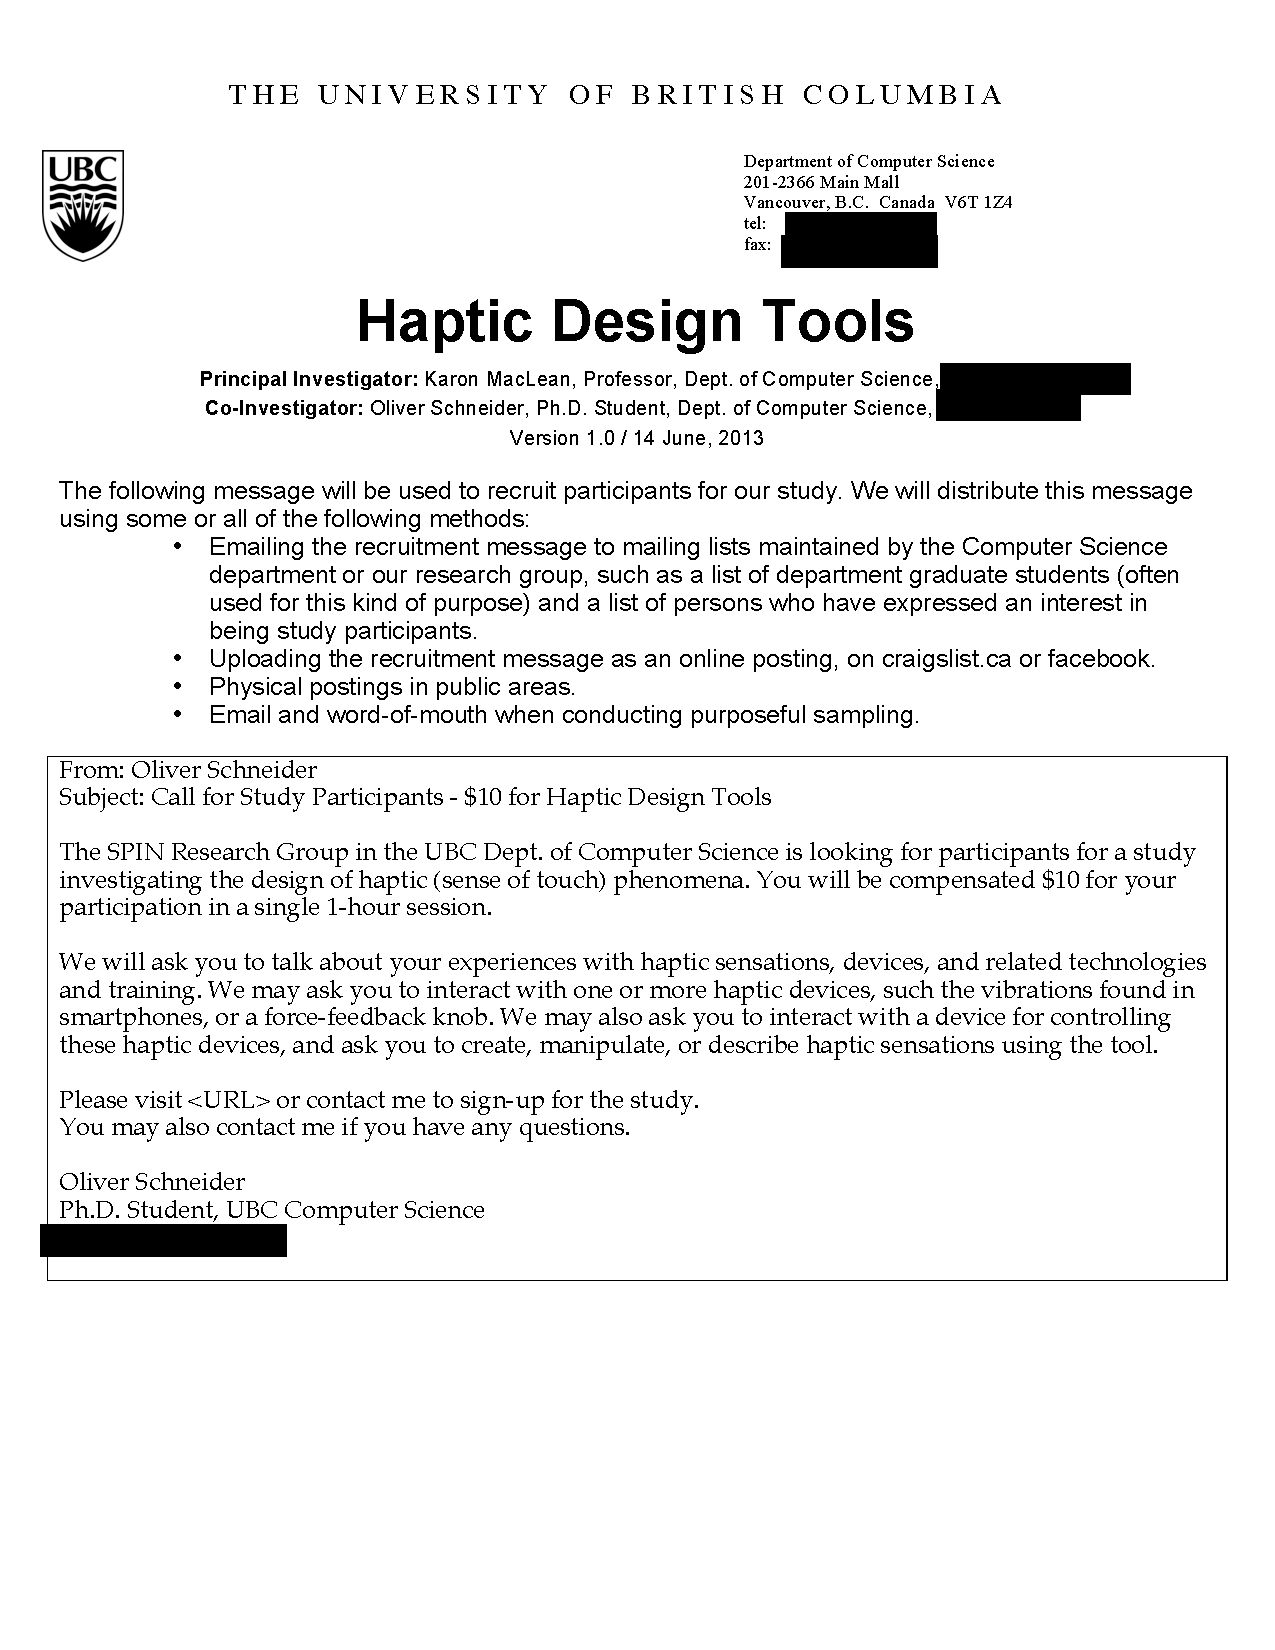
\includepdf[pages=-, pagecommand=\thispagestyle{plain}, width=1.25\textwidth]{Chapter99-SupportingMaterials/MainEthics/HapticDesignTools-CallForParticipation-v01-2013-06-14-anon}
	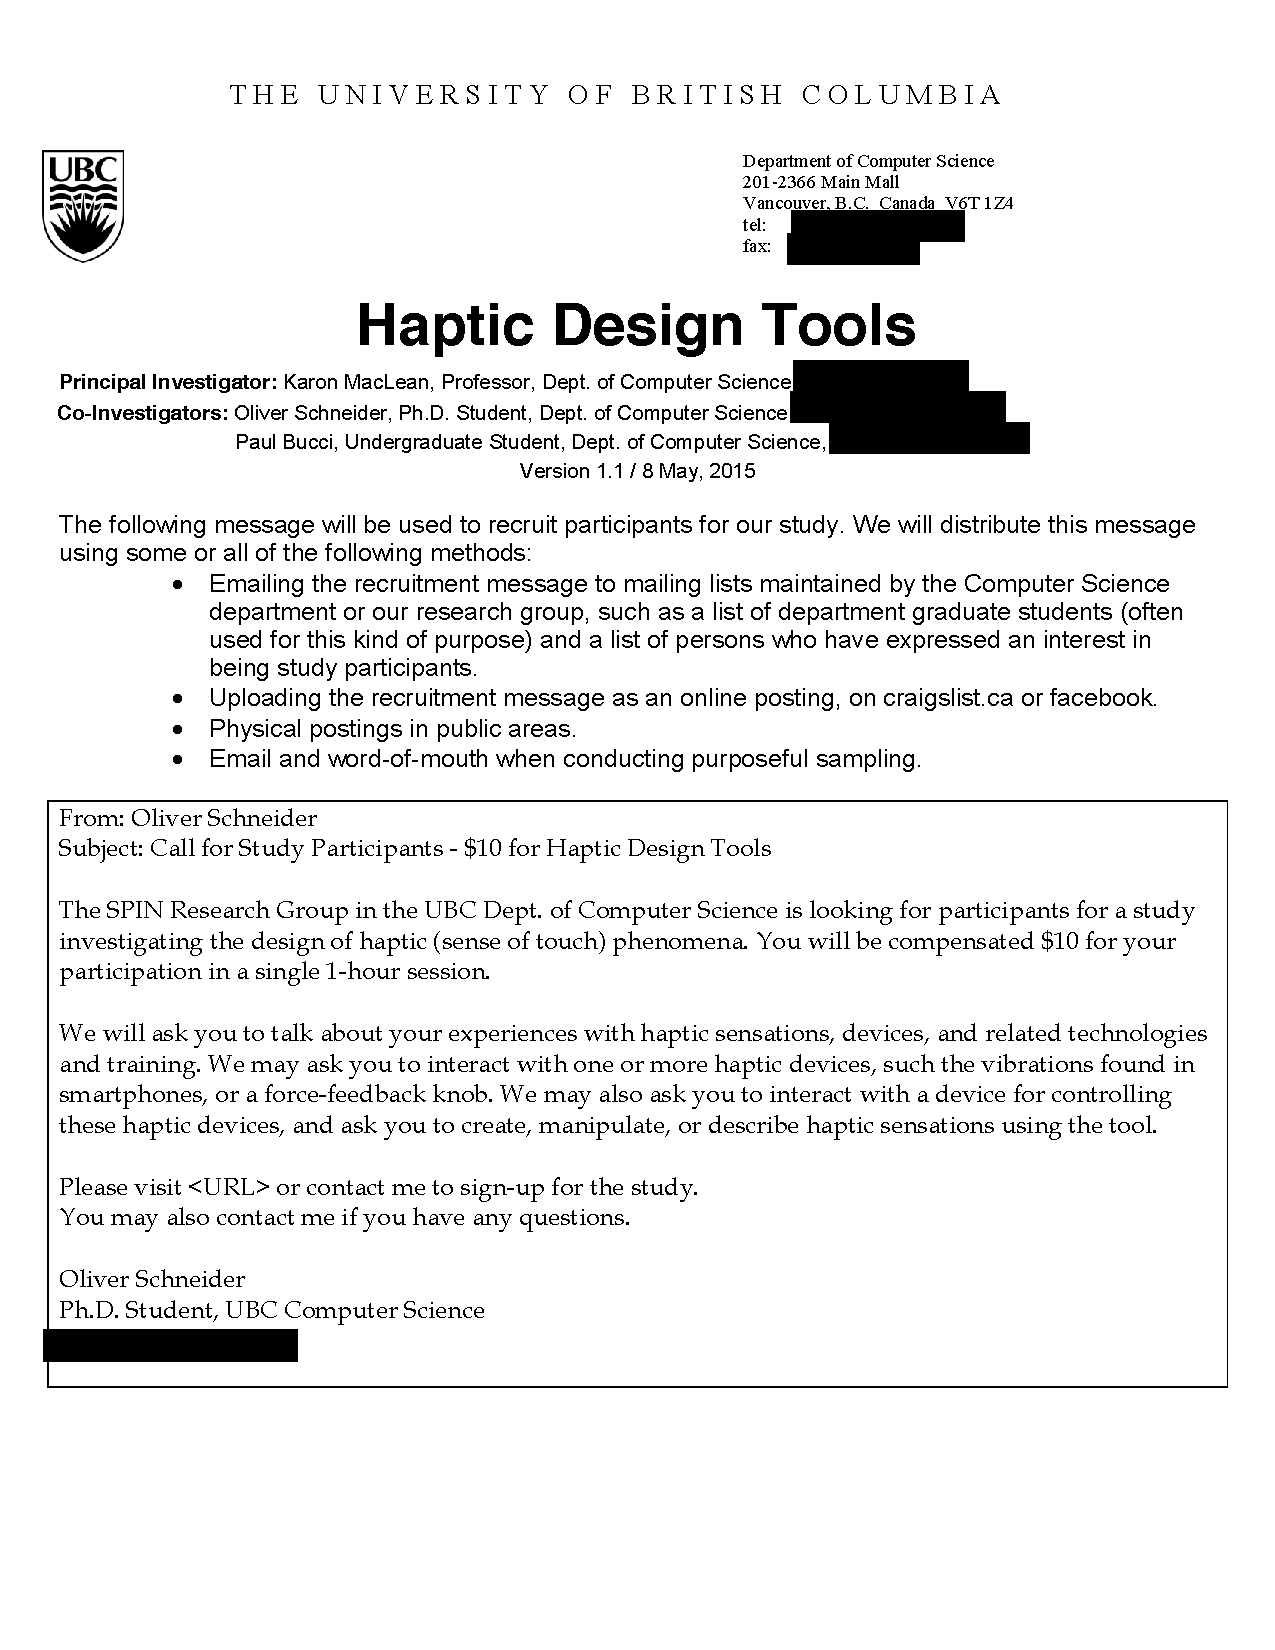
\includepdf[pages=-, pagecommand=\thispagestyle{plain}, width=1.25\textwidth]{Chapter99-SupportingMaterials/MainEthics/HapticDesignTools-CallForParticipation-v11-2015-05-08-anon}
	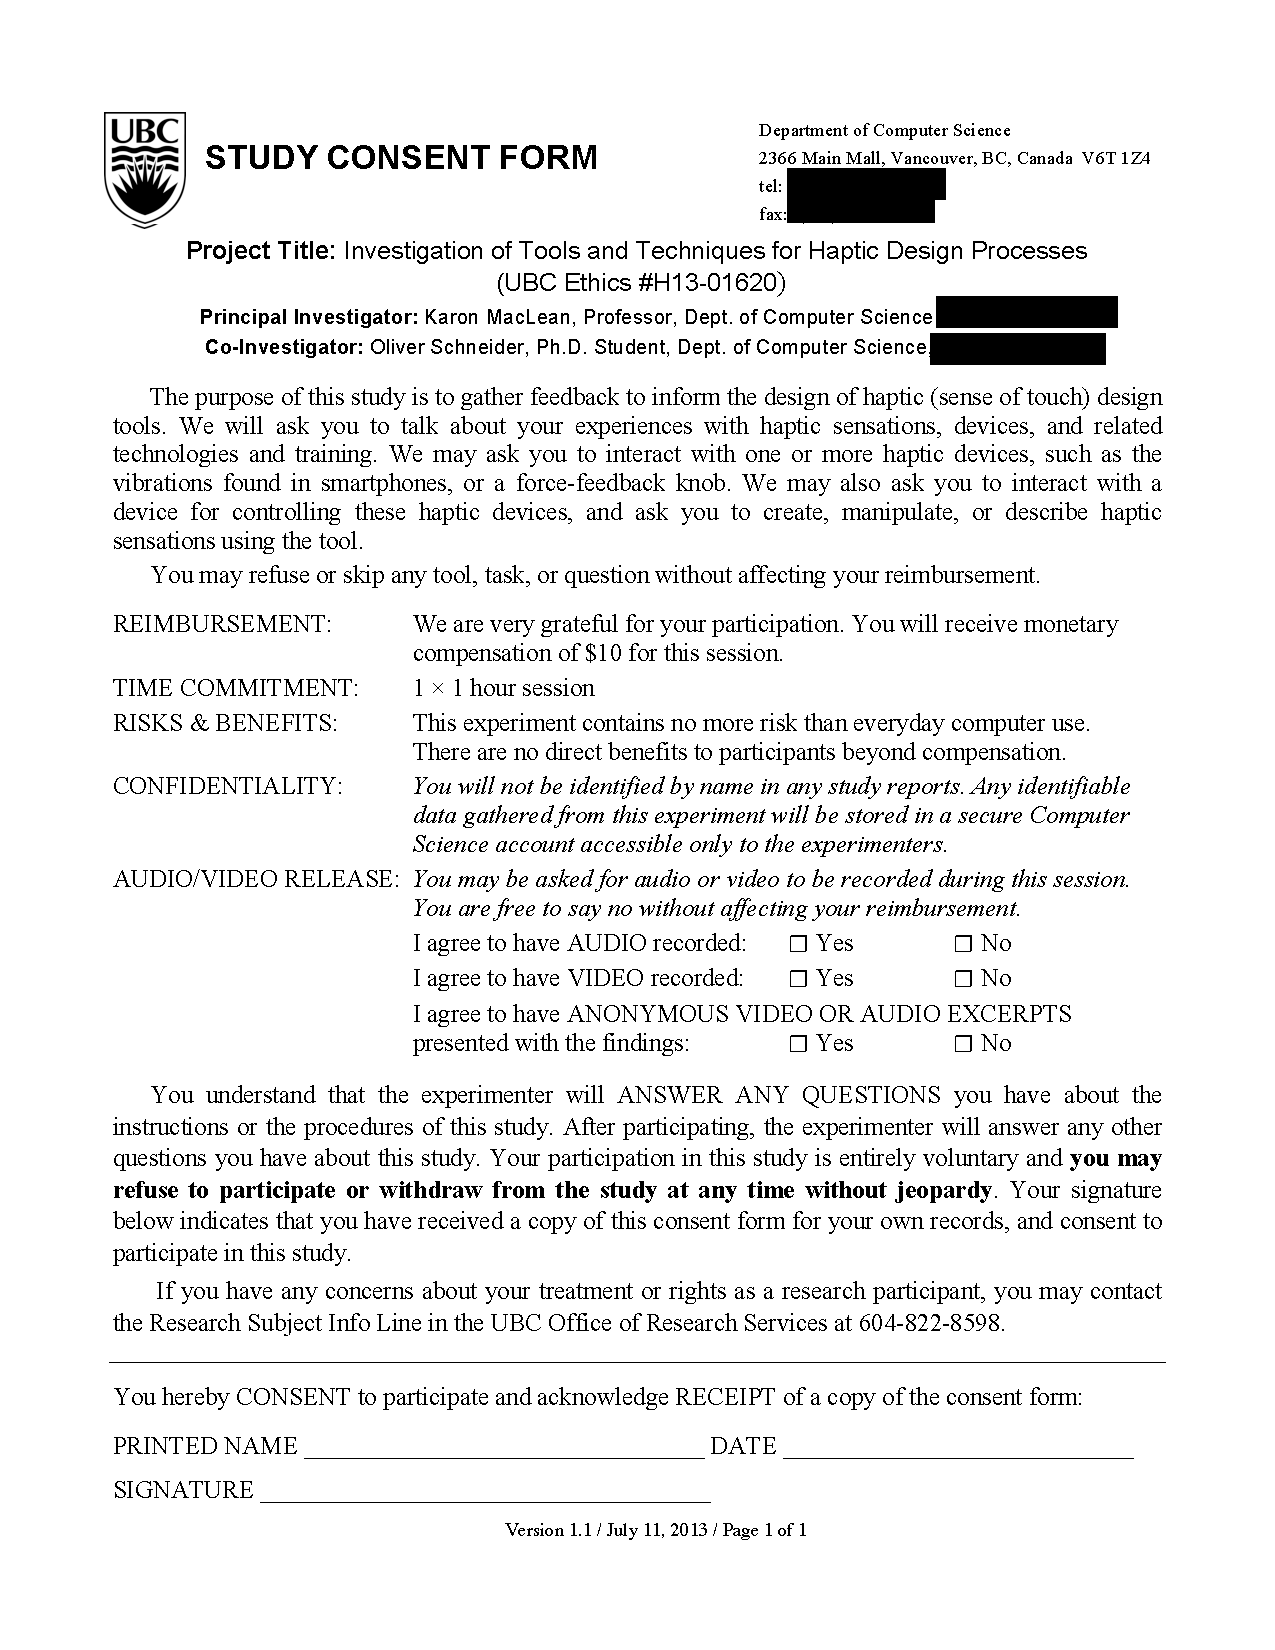
\includepdf[pages=-, pagecommand=\thispagestyle{plain}, width=1.25\textwidth]{Chapter99-SupportingMaterials/MainEthics/HapticDesignTools-Consent-v11-2013-07-11-anon}
	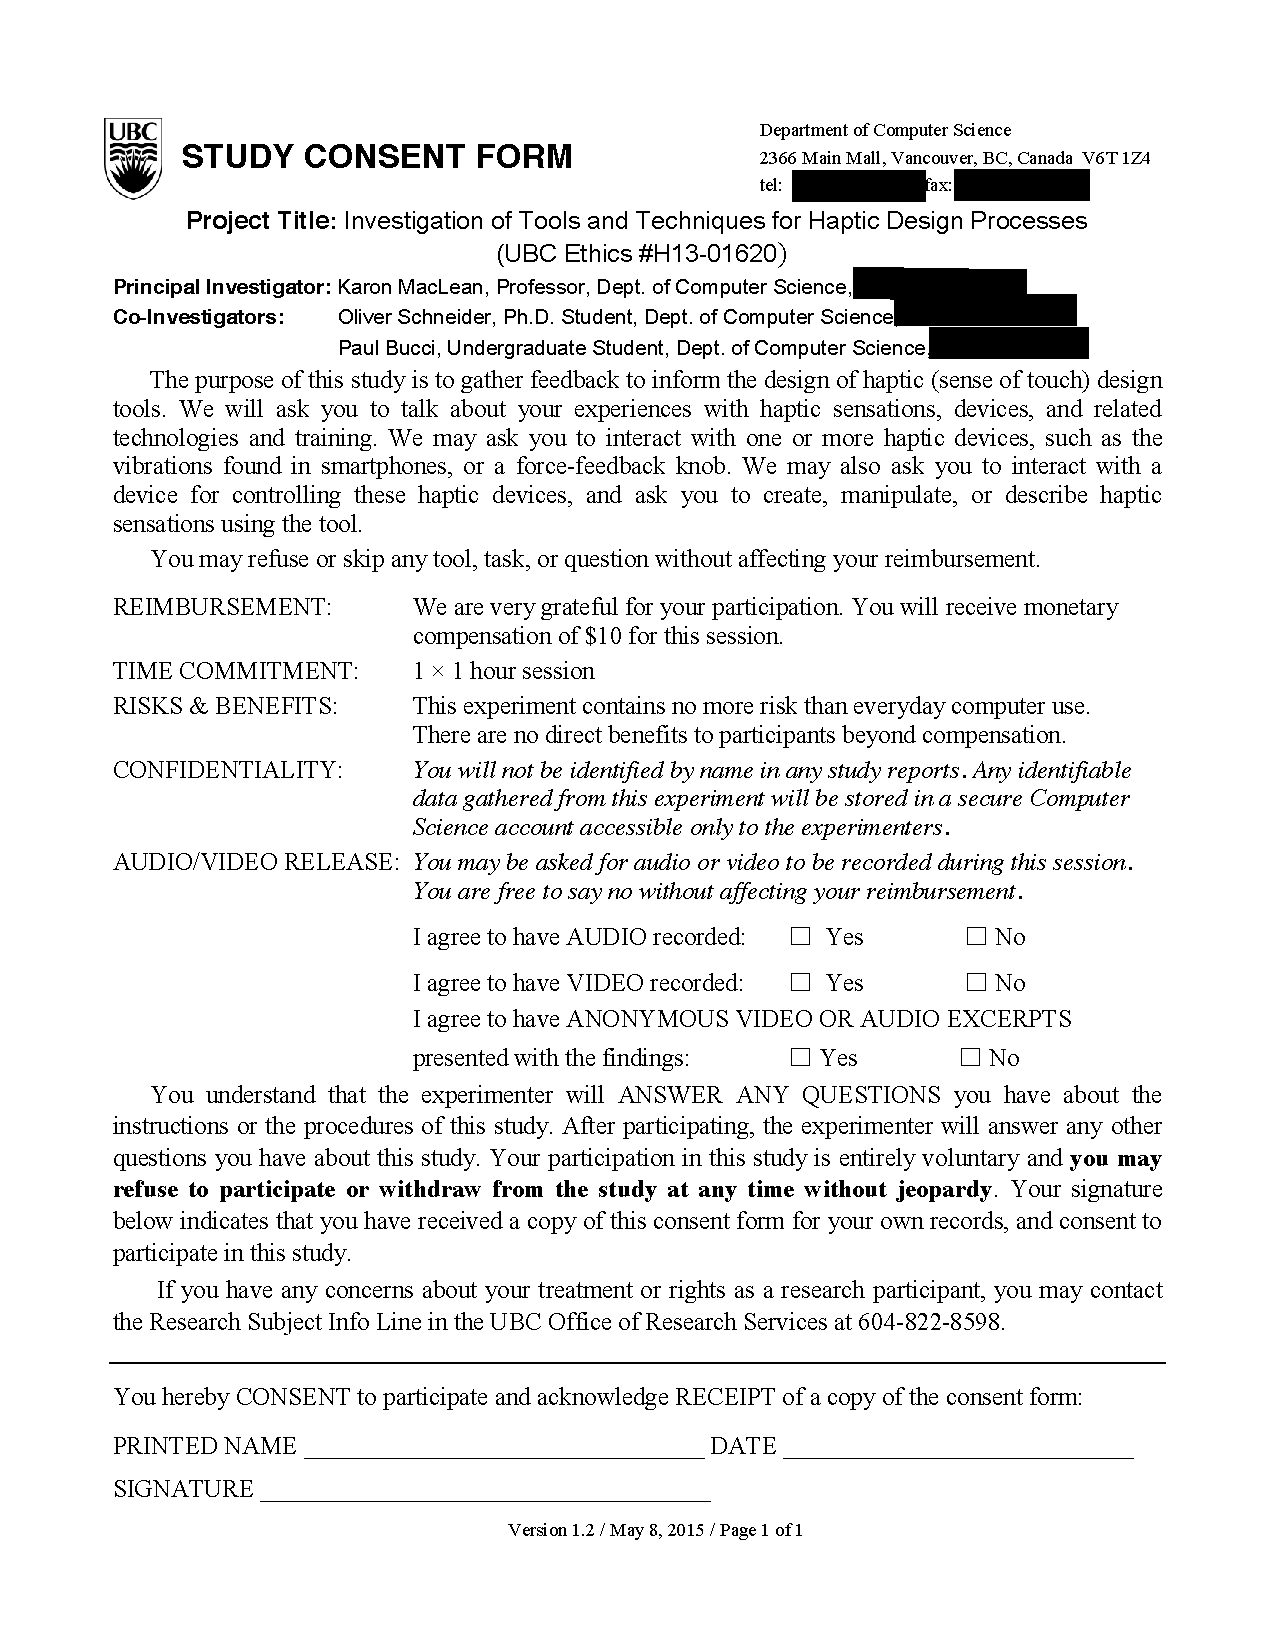
\includepdf[pages=-, pagecommand=\thispagestyle{plain}, width=1.25\textwidth]{Chapter99-SupportingMaterials/MainEthics/HapticDesignTools-Consent-v12-2015-05-08-anon}
	
\includepdf[pages=-, pagecommand=\thispagestyle{plain}, width=1.25\textwidth]{Chapter99-SupportingMaterials/MainEthics/HapticDesignTools-RequestForFollowup-v01-2013-6-27-anon}
	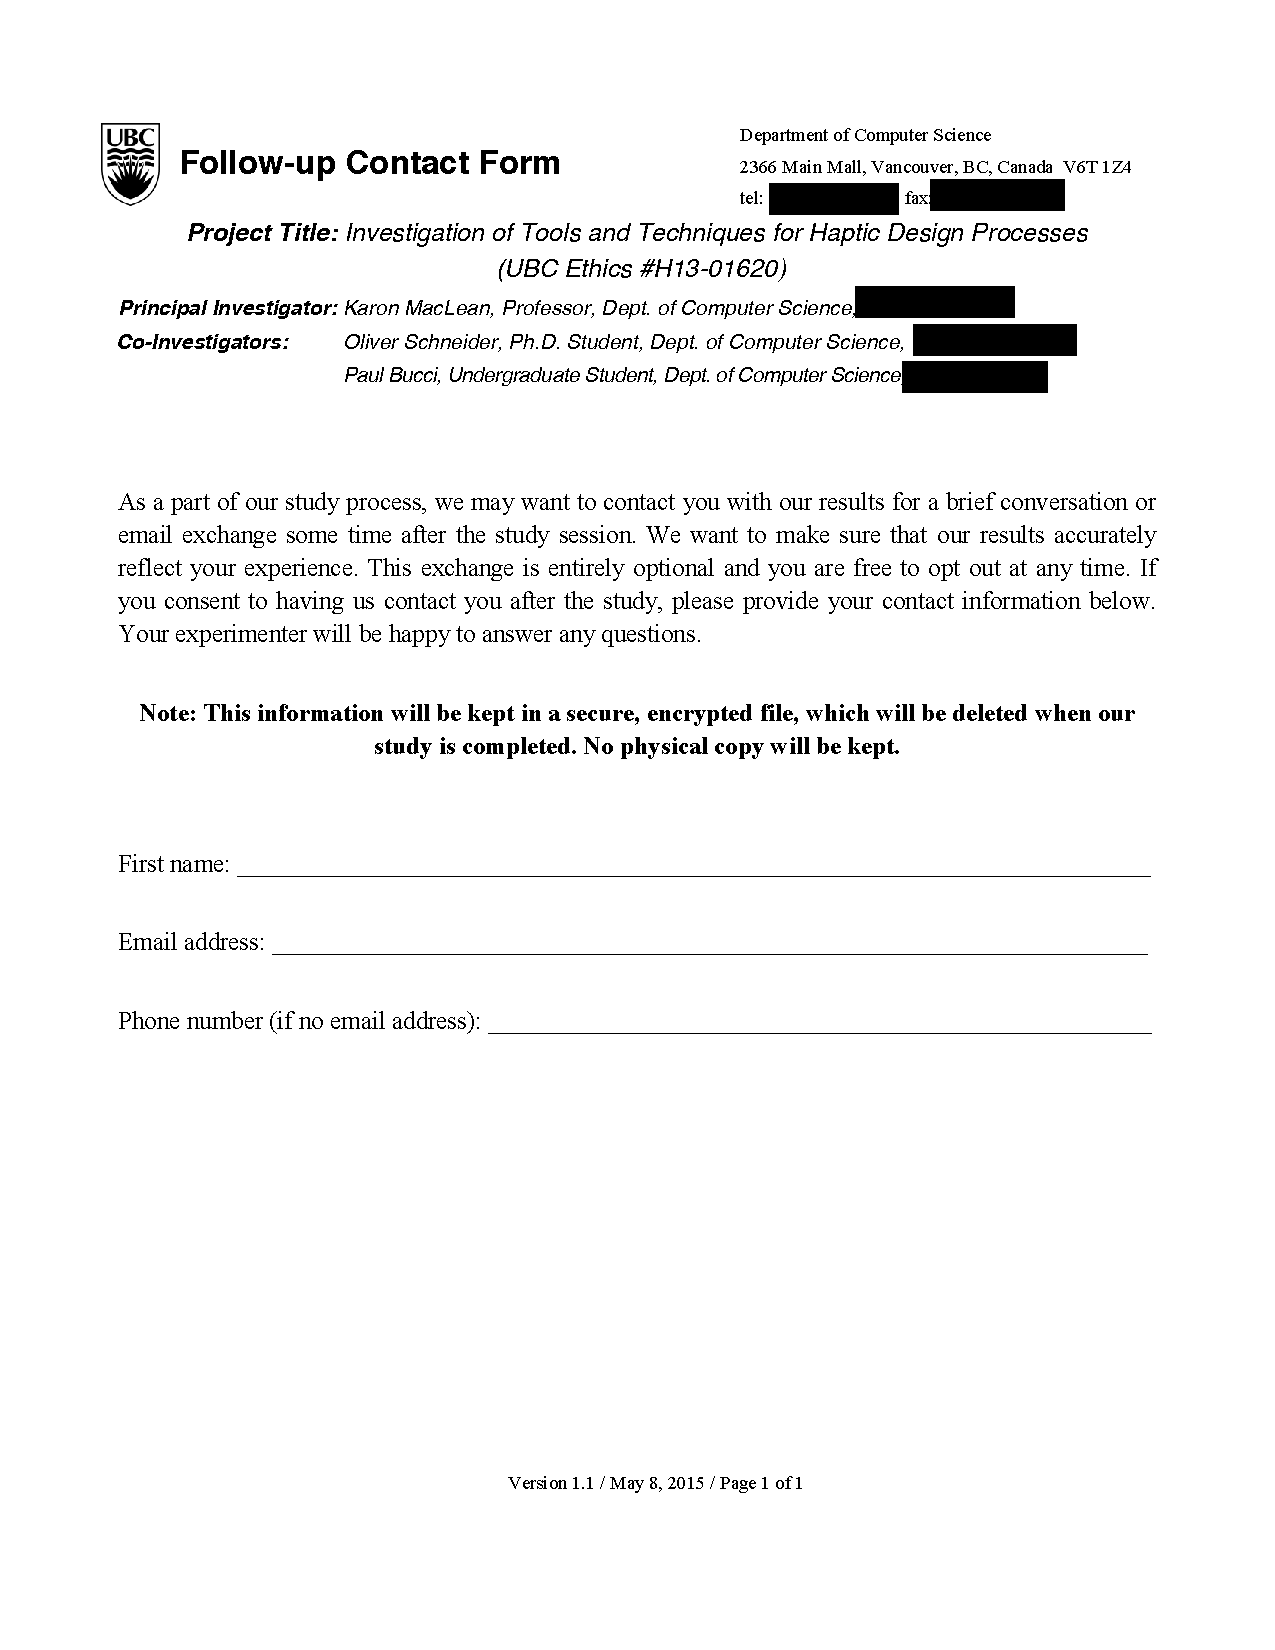
\includepdf[pages=-, pagecommand=\thispagestyle{plain}, width=1.25\textwidth]{Chapter99-SupportingMaterials/MainEthics/HapticDesignTools-RequestForFollowup-v11-2015-5-8-anon}



	%tactile animation
	\subsection{Tactile Animation Forms}
	\label{ch:SupportingMaterials:ConsentForms:TactileAnimation}
	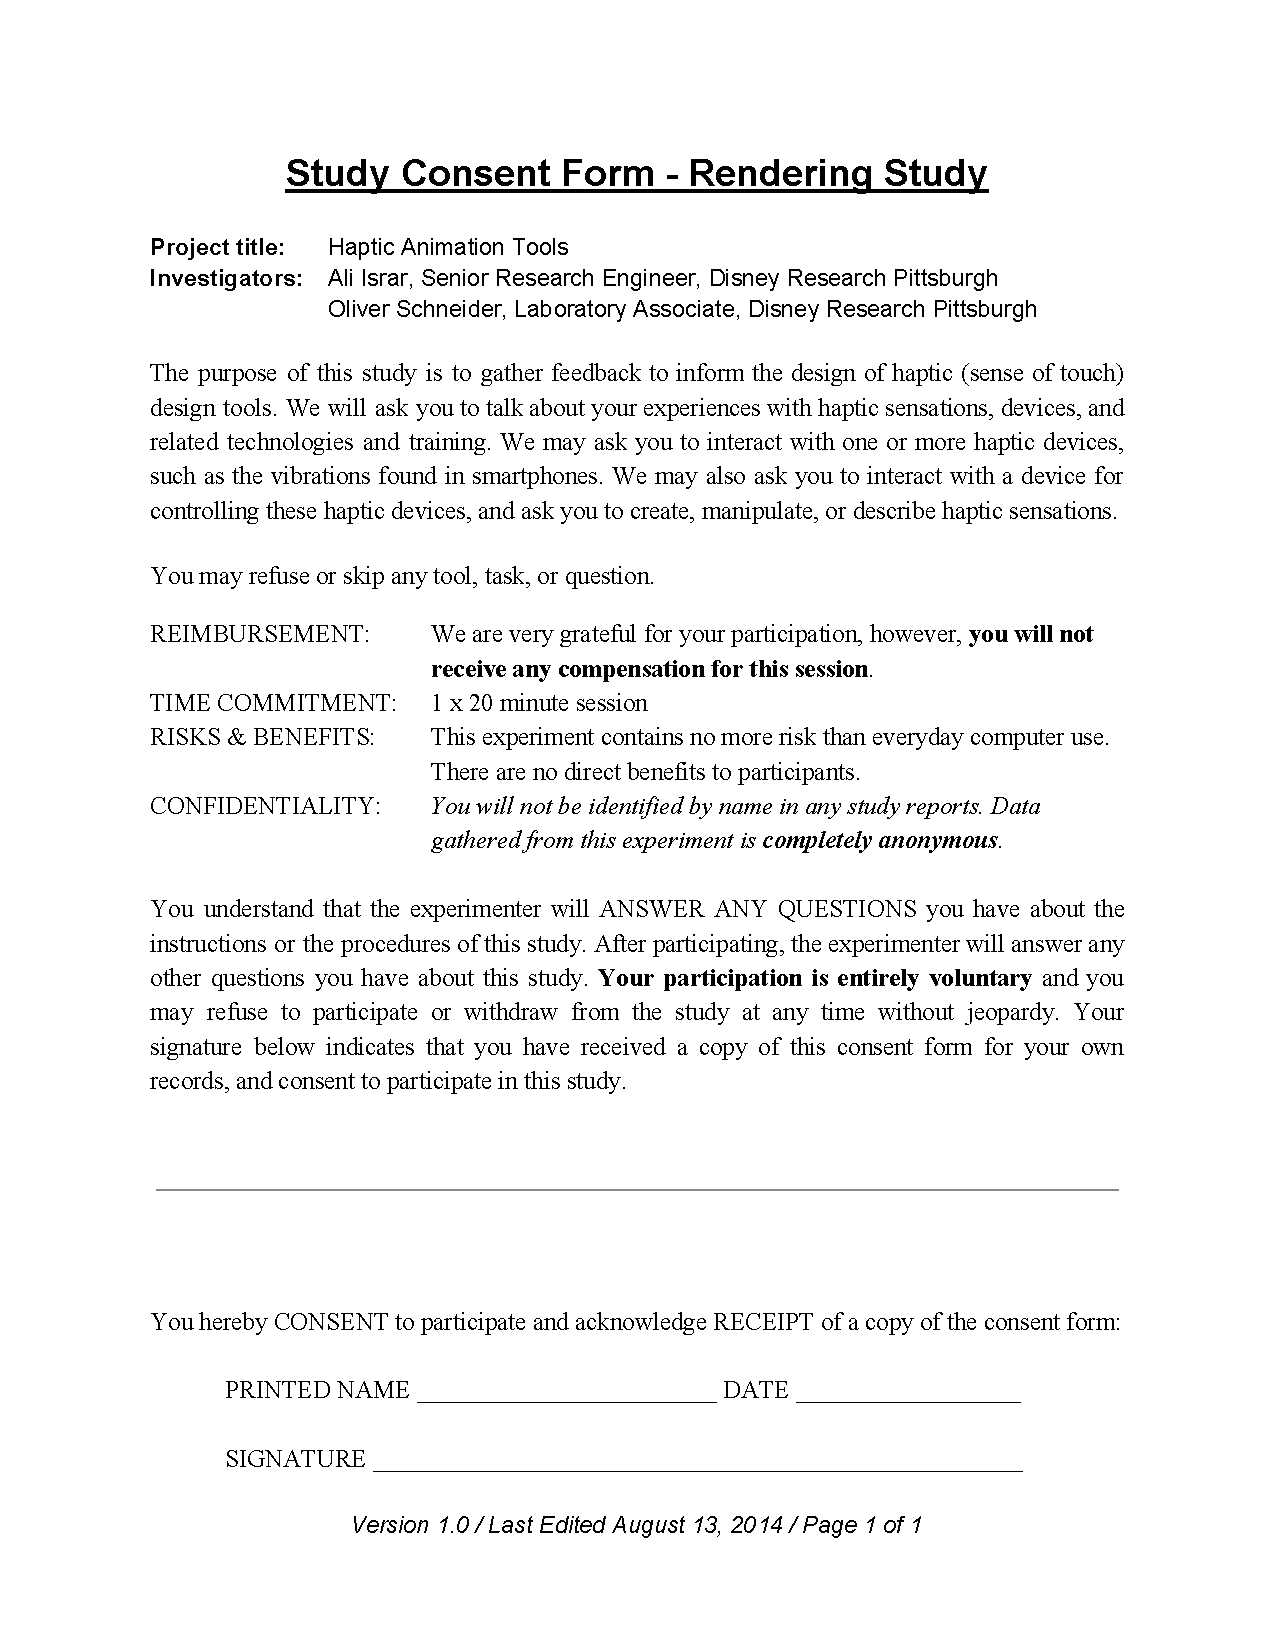
\includepdf[pages=-, pagecommand=\thispagestyle{plain}, width=1.25\textwidth]{Chapter99-SupportingMaterials/MainEthics/HapticAnimationConsentForm-RenderingStudy}
	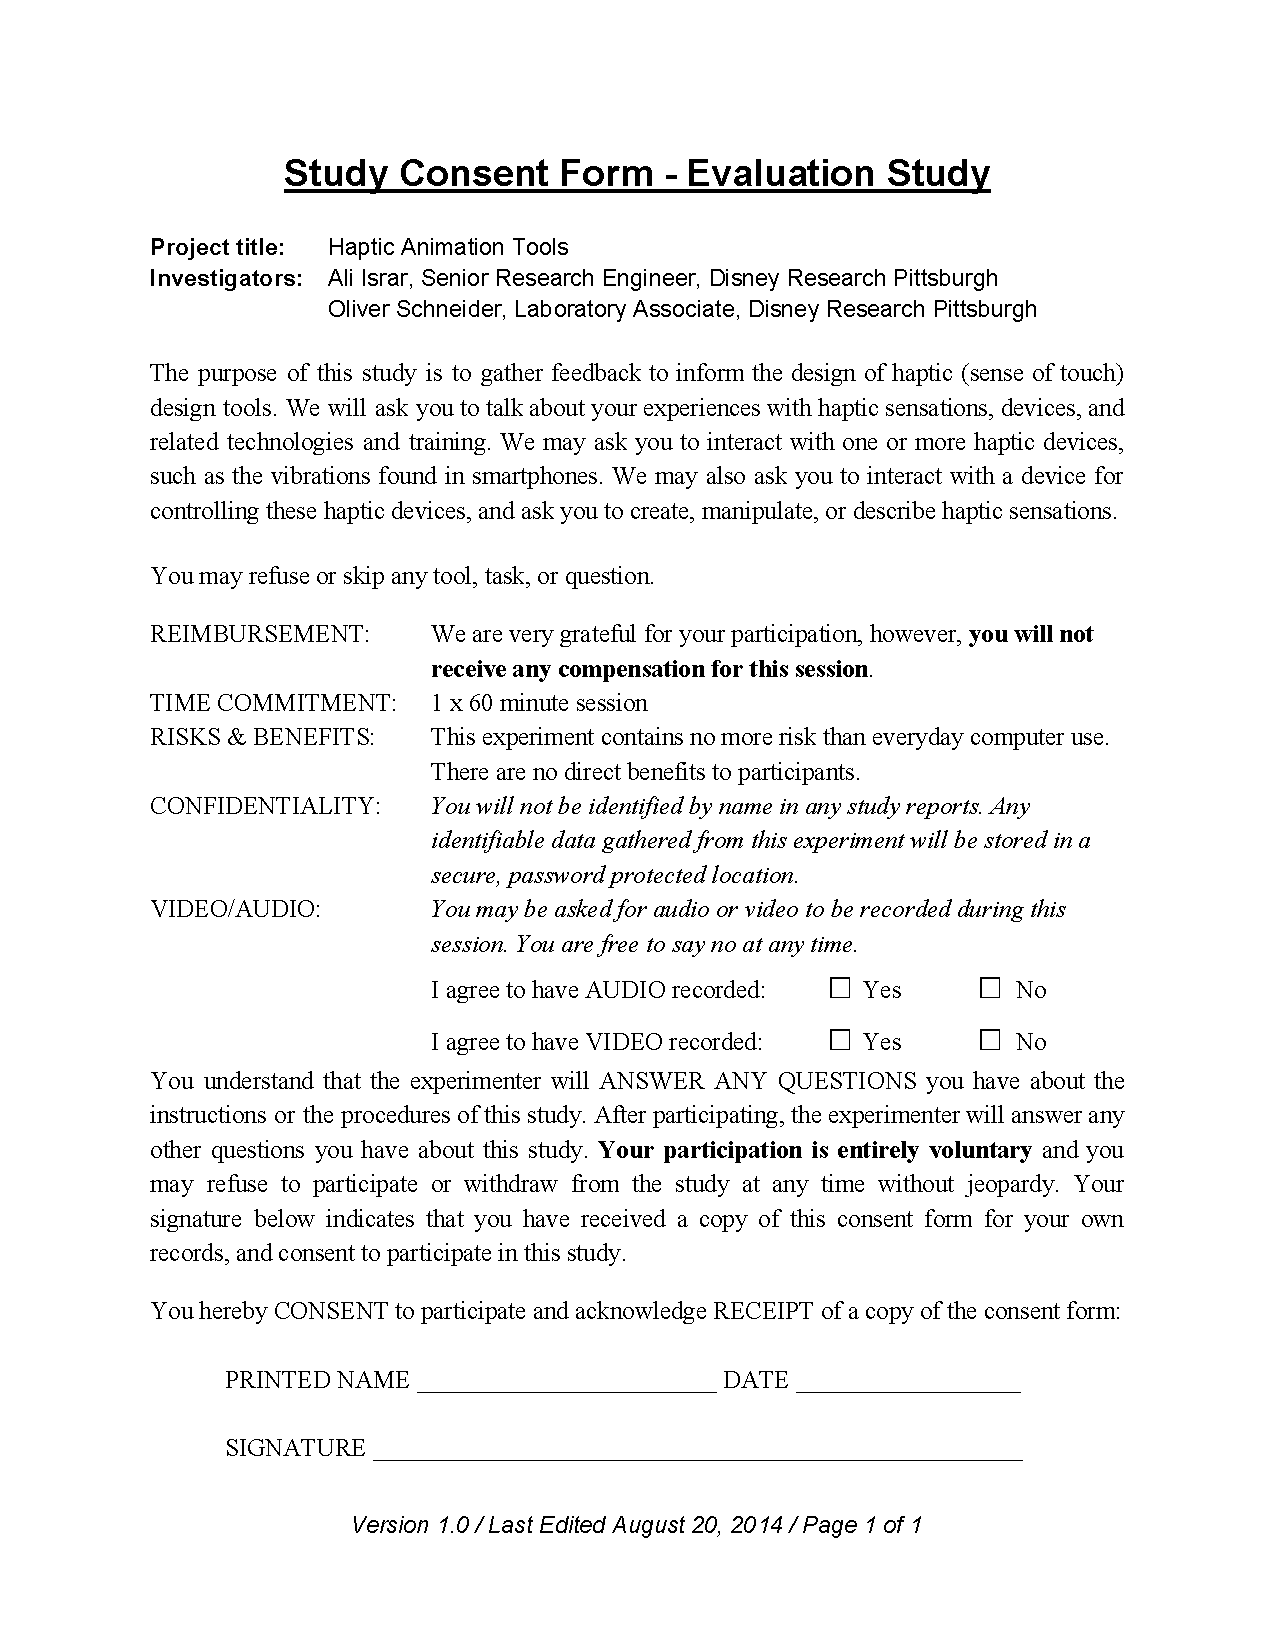
\includepdf[pages=-, pagecommand=\thispagestyle{plain}, width=1.25\textwidth]{Chapter99-SupportingMaterials/MainEthics/HapticAnimationConsentForm-EvaluationStudy}
	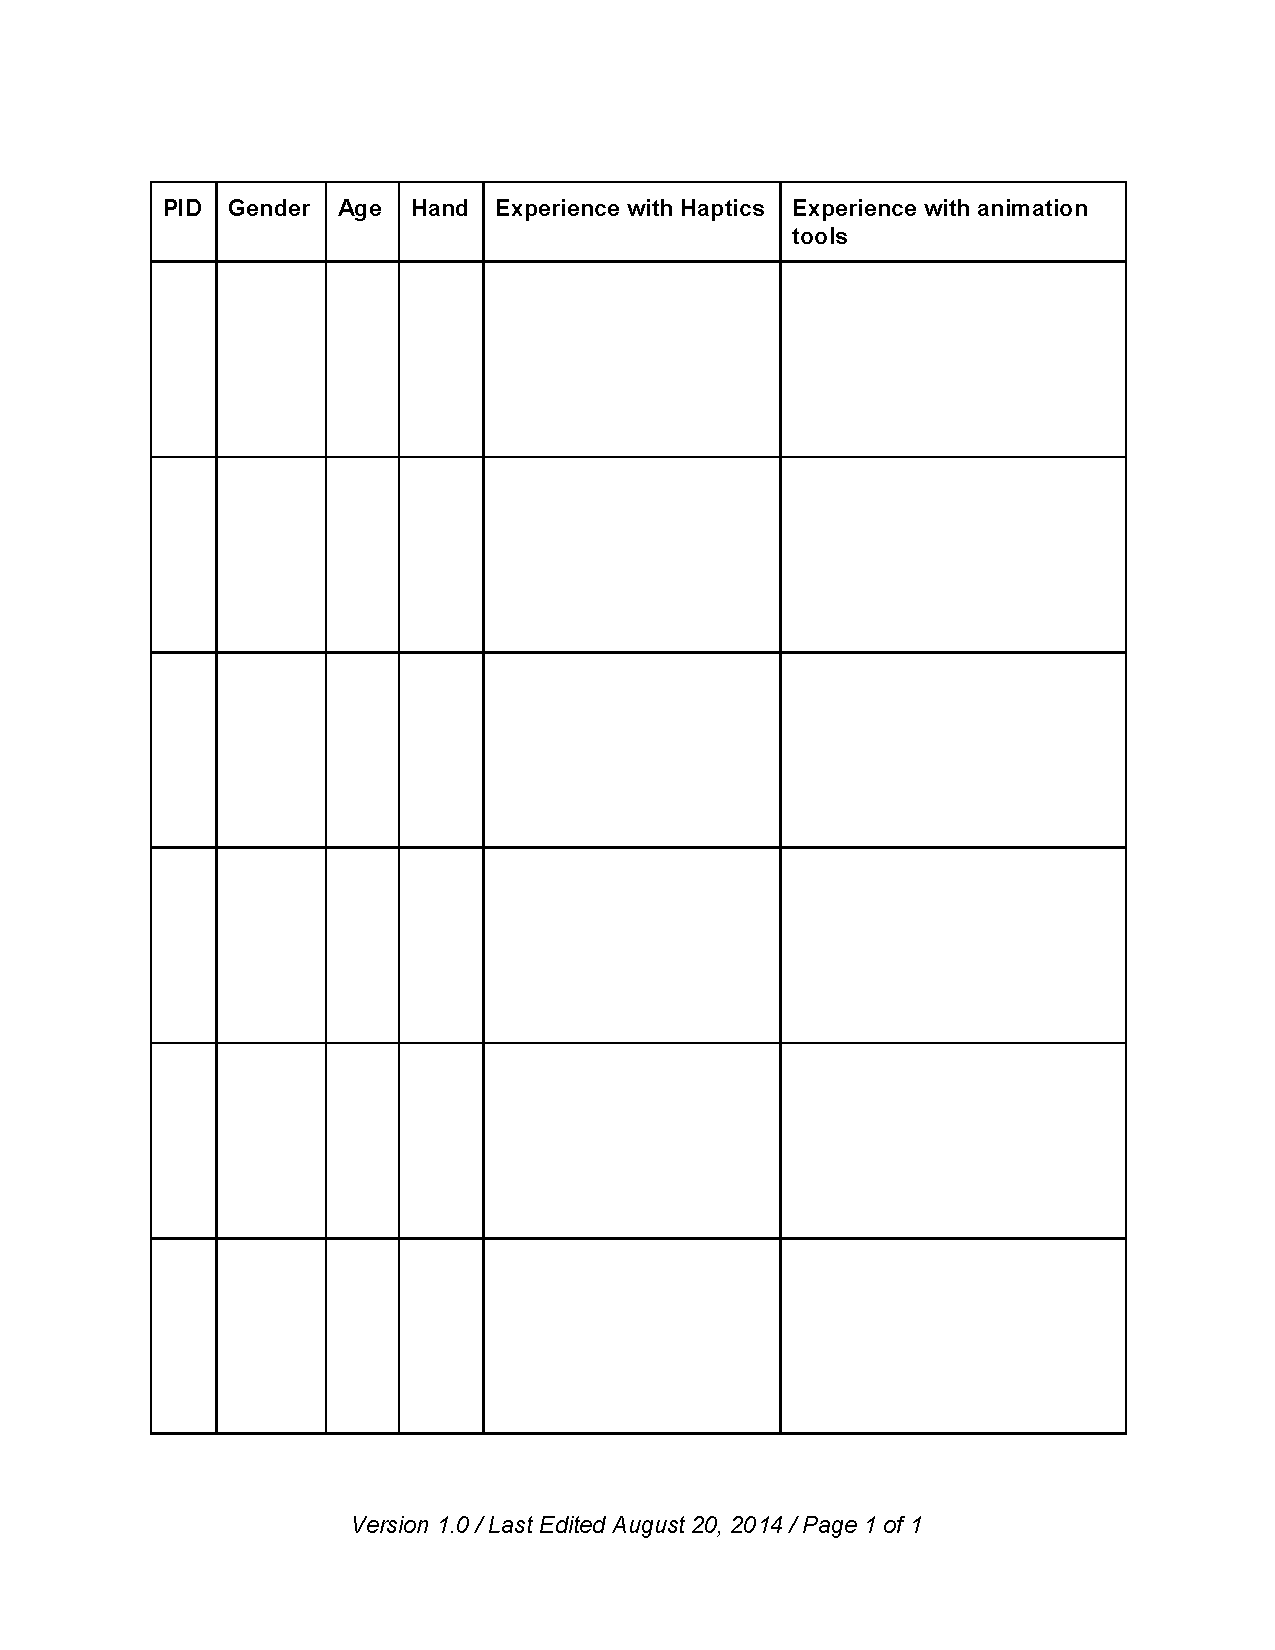
\includepdf[pages=-, pagecommand=\thispagestyle{plain}, width=1.25\textwidth]{Chapter99-SupportingMaterials/MainEthics/HapticAnimationDemographicsSheet}
%	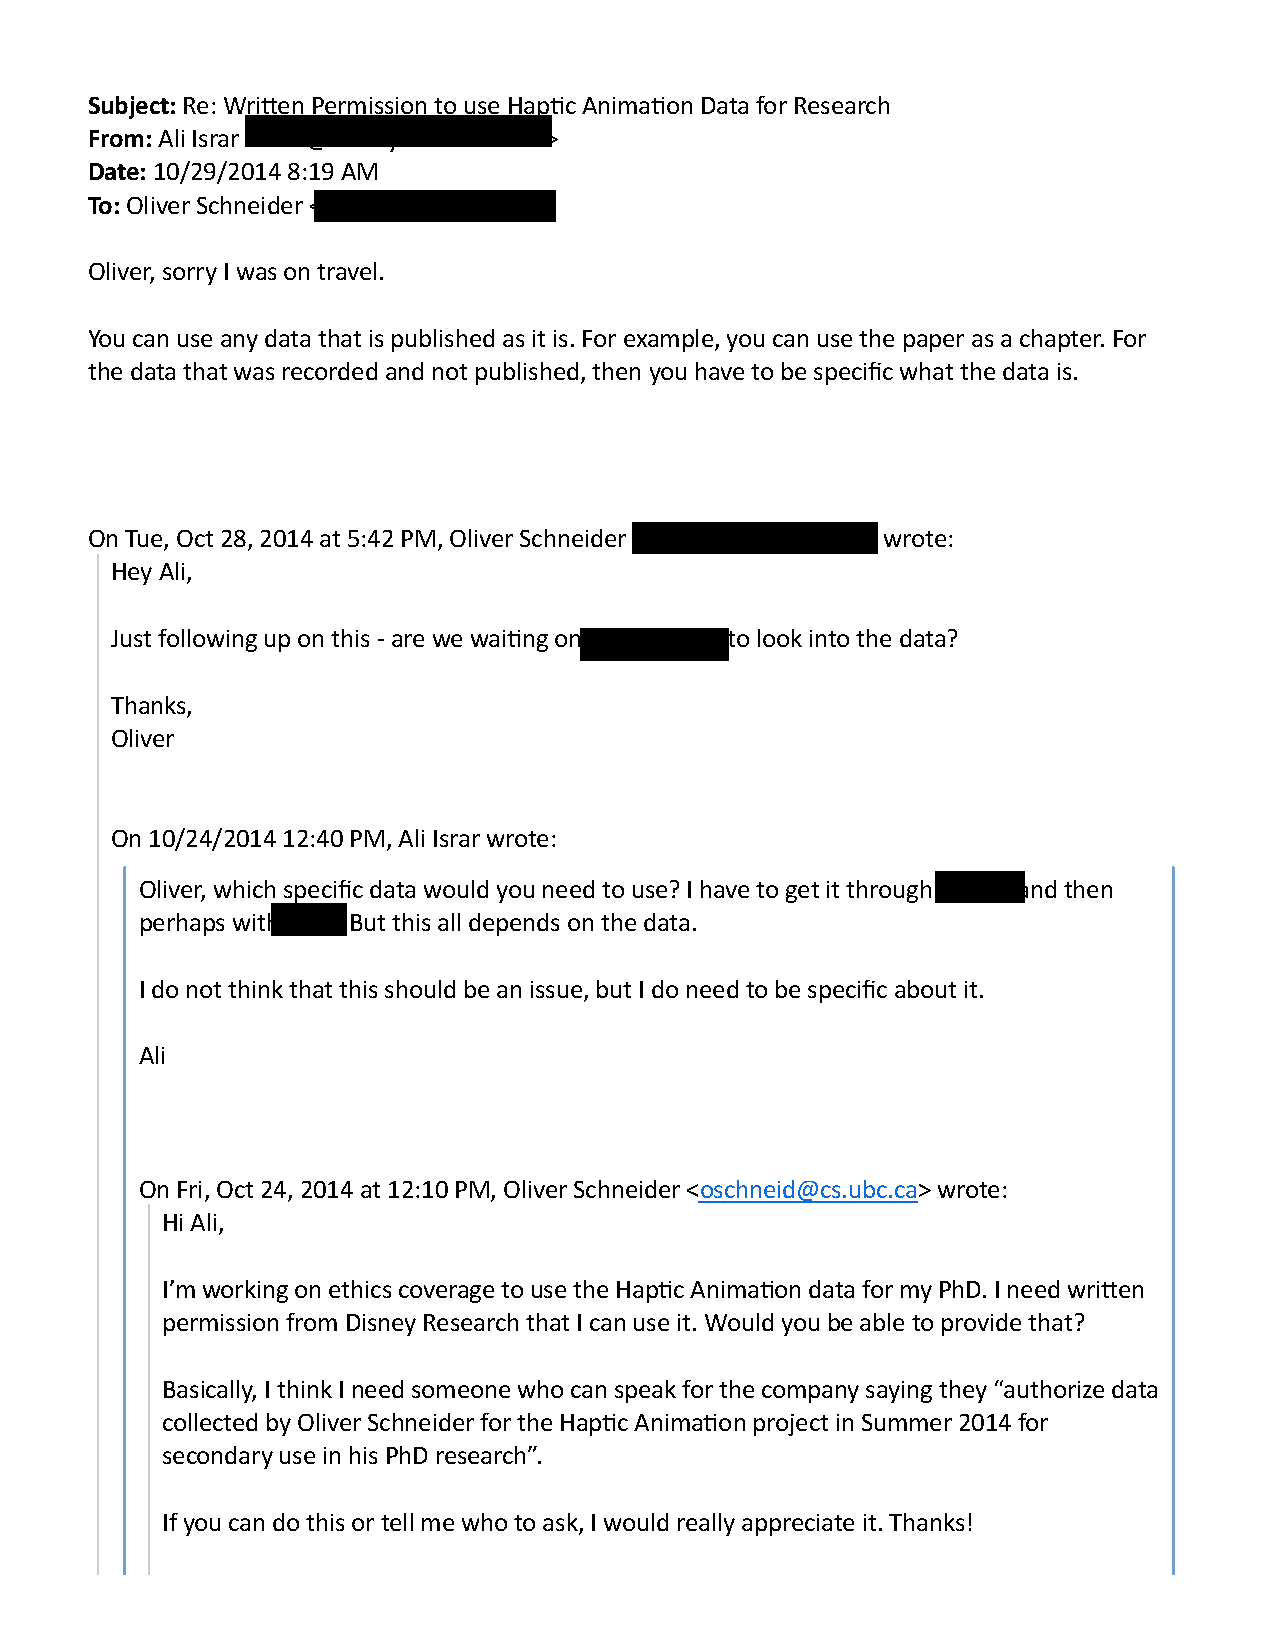
\includepdf[pages=-, pagecommand=\thispagestyle{plain}, width=1.25\textwidth]{Chapter99-SupportingMaterials/MainEthics/WrittenPermissiontouseHapticAnimationDataforResearch-anon}
	
	
	%haptician interviews
	\subsection{HapTurk Forms}
	\label{ch:SupportingMaterials:ConsentForms:HapTurk}
	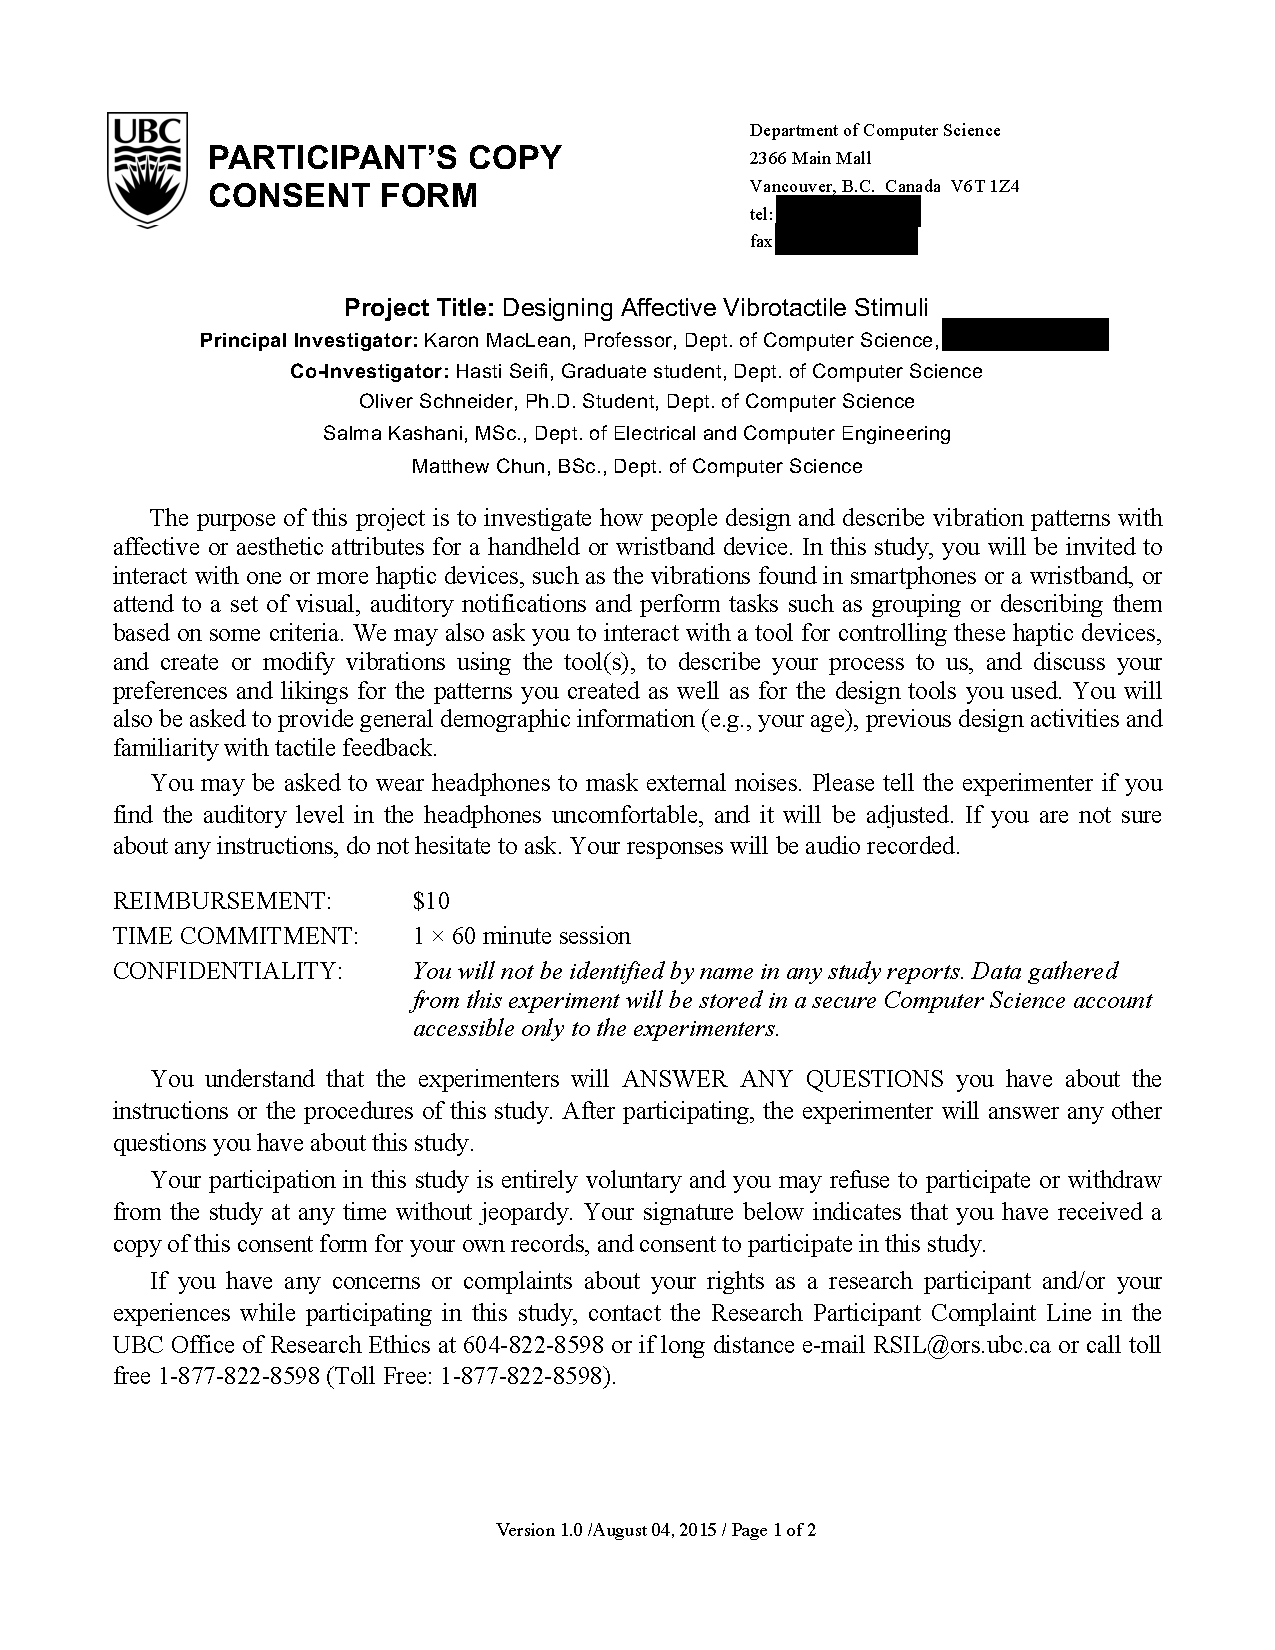
\includepdf[pages=-, pagecommand=\thispagestyle{plain}, width=1.25\textwidth]{Chapter99-SupportingMaterials/HSEthics/HapTurk-fromHS/AnnotationStudyConsentForm_v10-anon}
	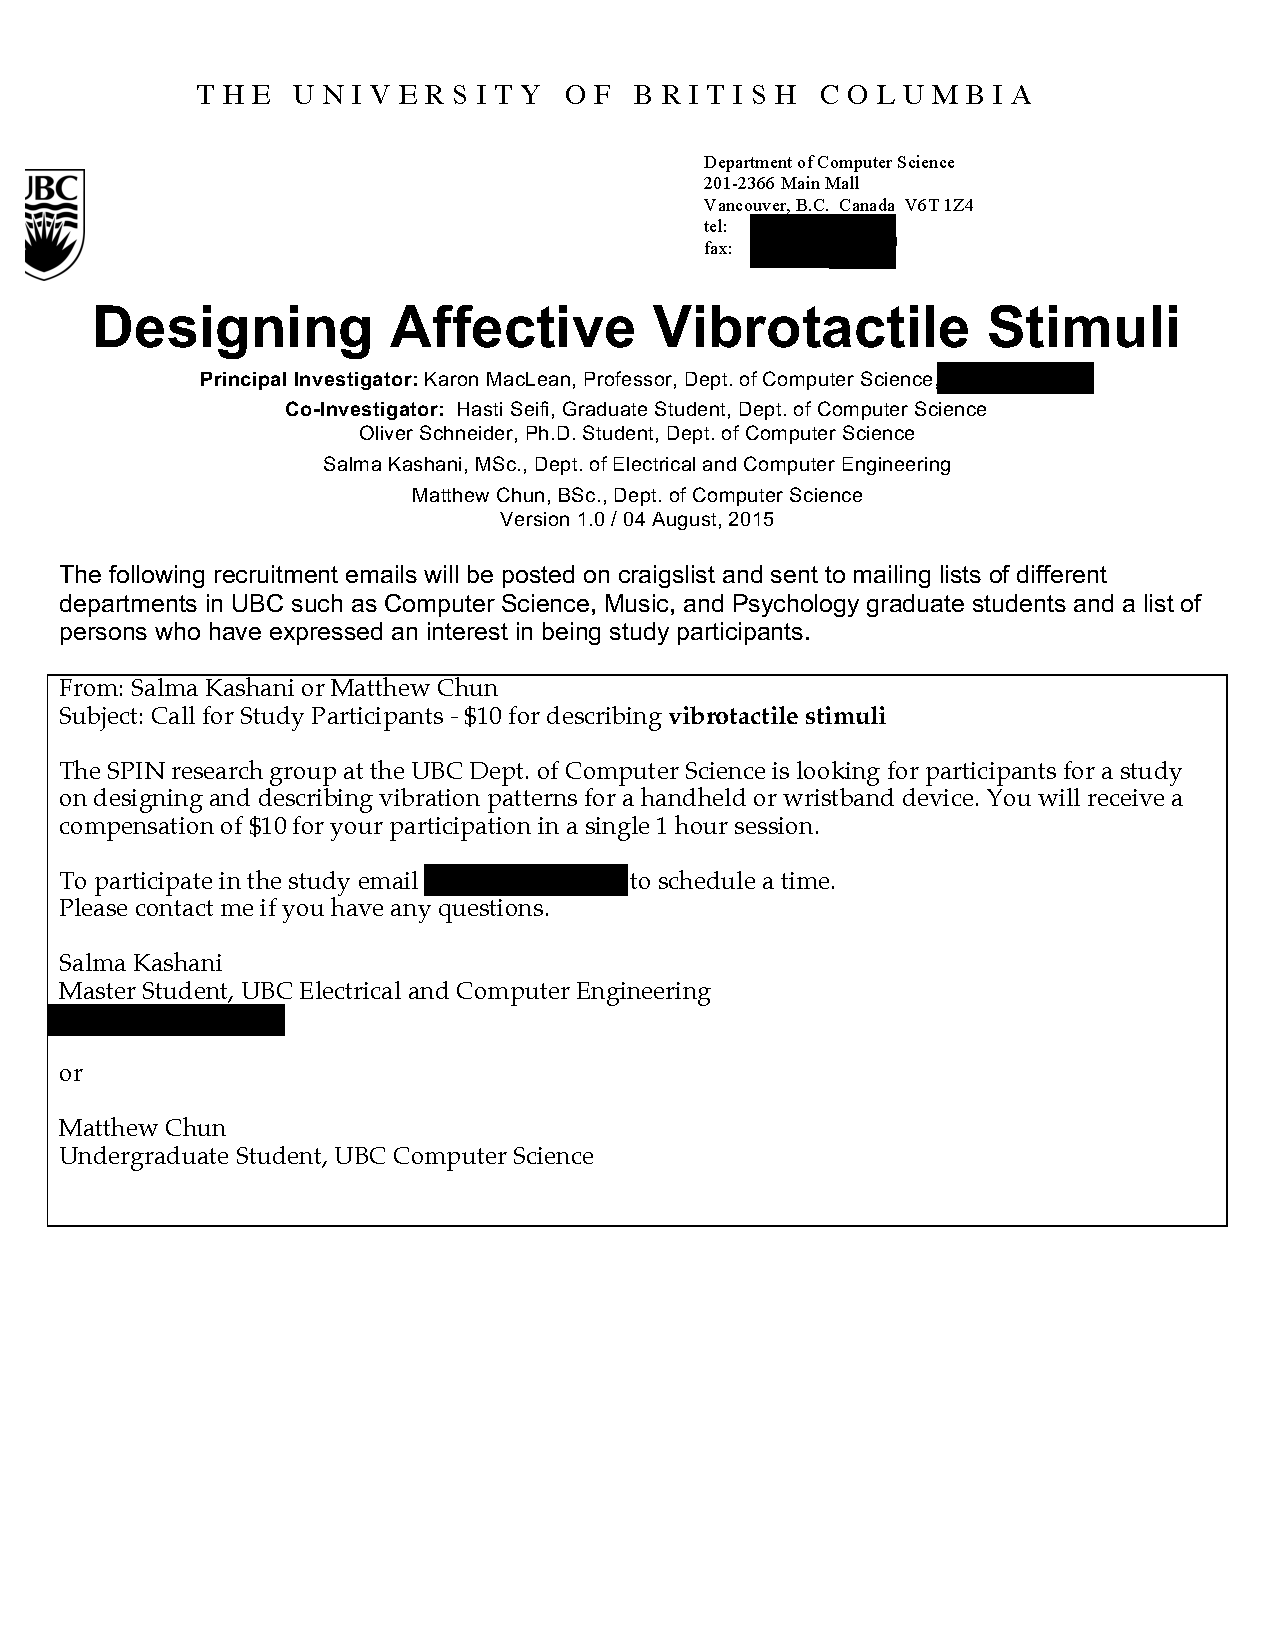
\includepdf[pages=-, pagecommand=\thispagestyle{plain}, width=1.25\textwidth]{Chapter99-SupportingMaterials/HSEthics/HapTurk-fromHS/AnnotationStudyRecruitmentEmail_v10-anon}
	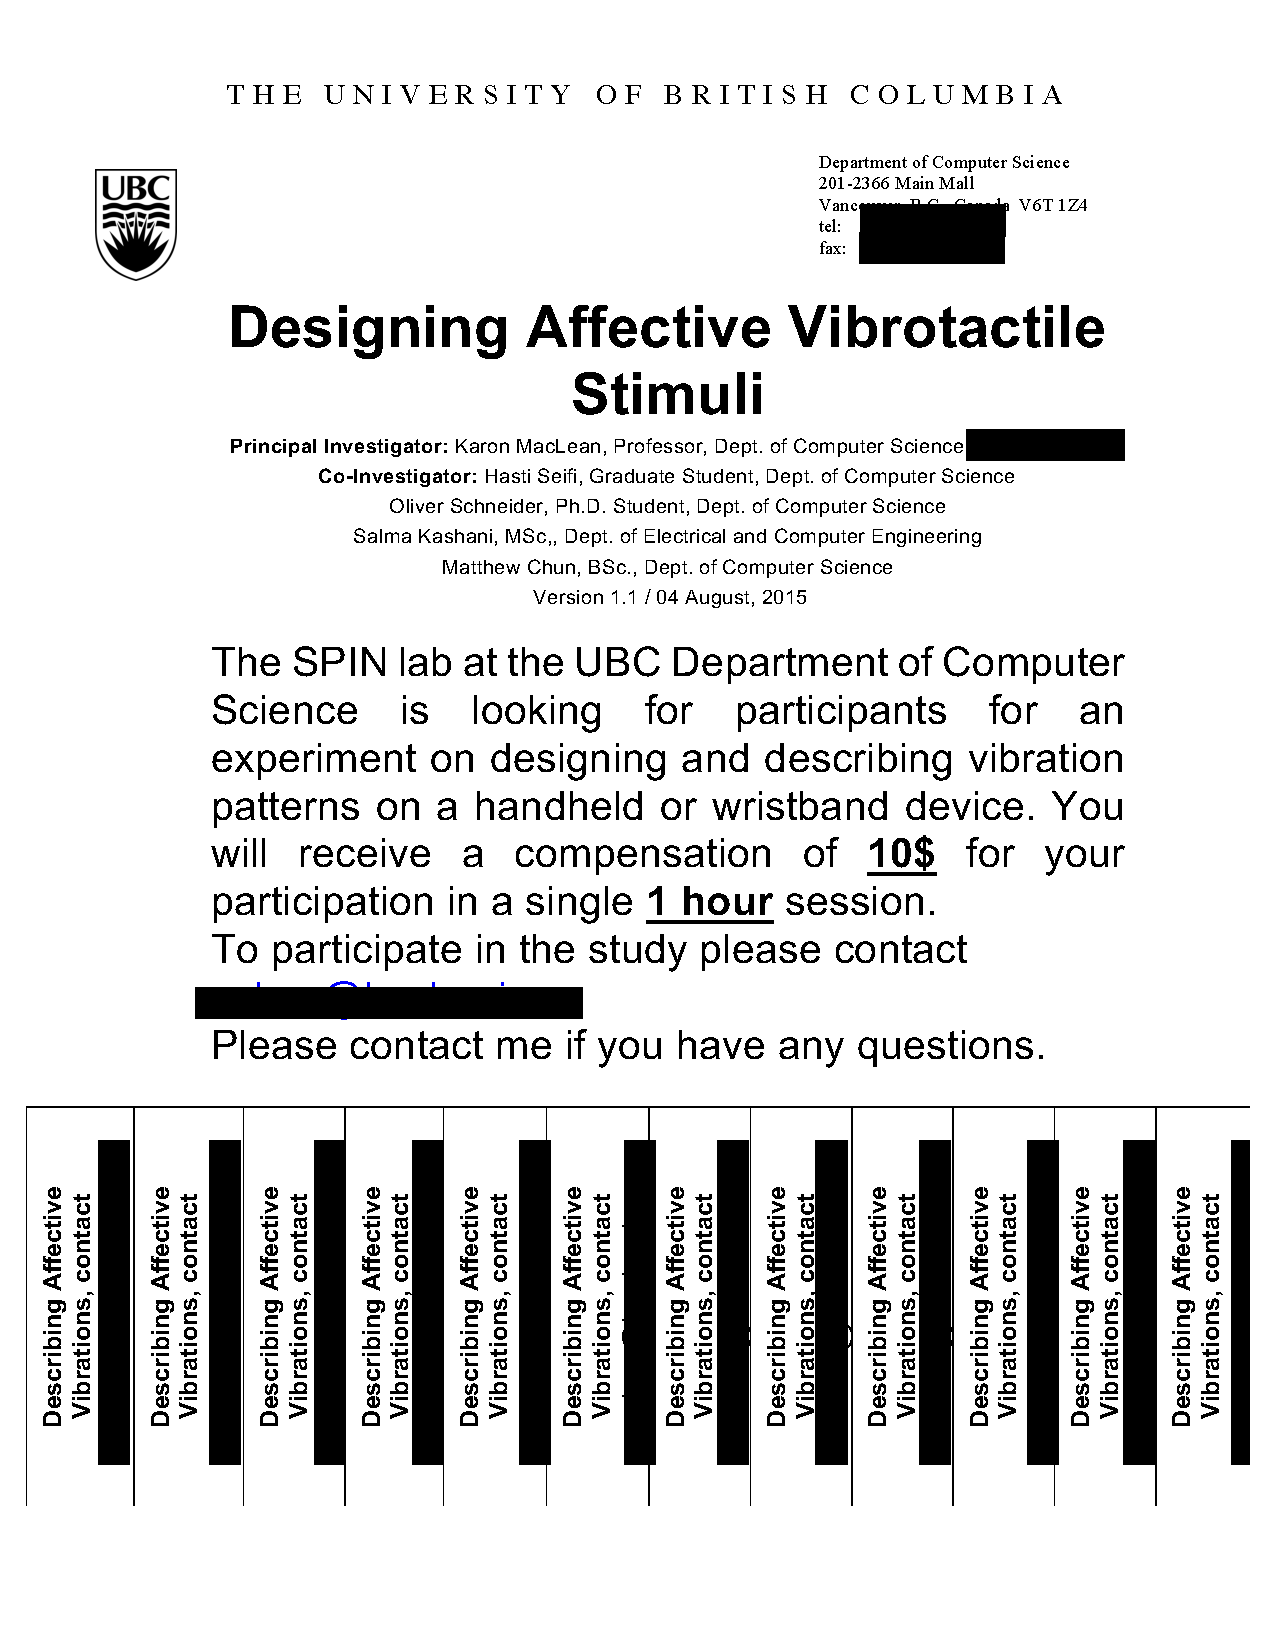
\includepdf[pages=-, pagecommand=\thispagestyle{plain}, width=1.25\textwidth]{Chapter99-SupportingMaterials/HSEthics/HapTurk-fromHS/AnnotationStudyRecruitmentPoster_v11-anon}
	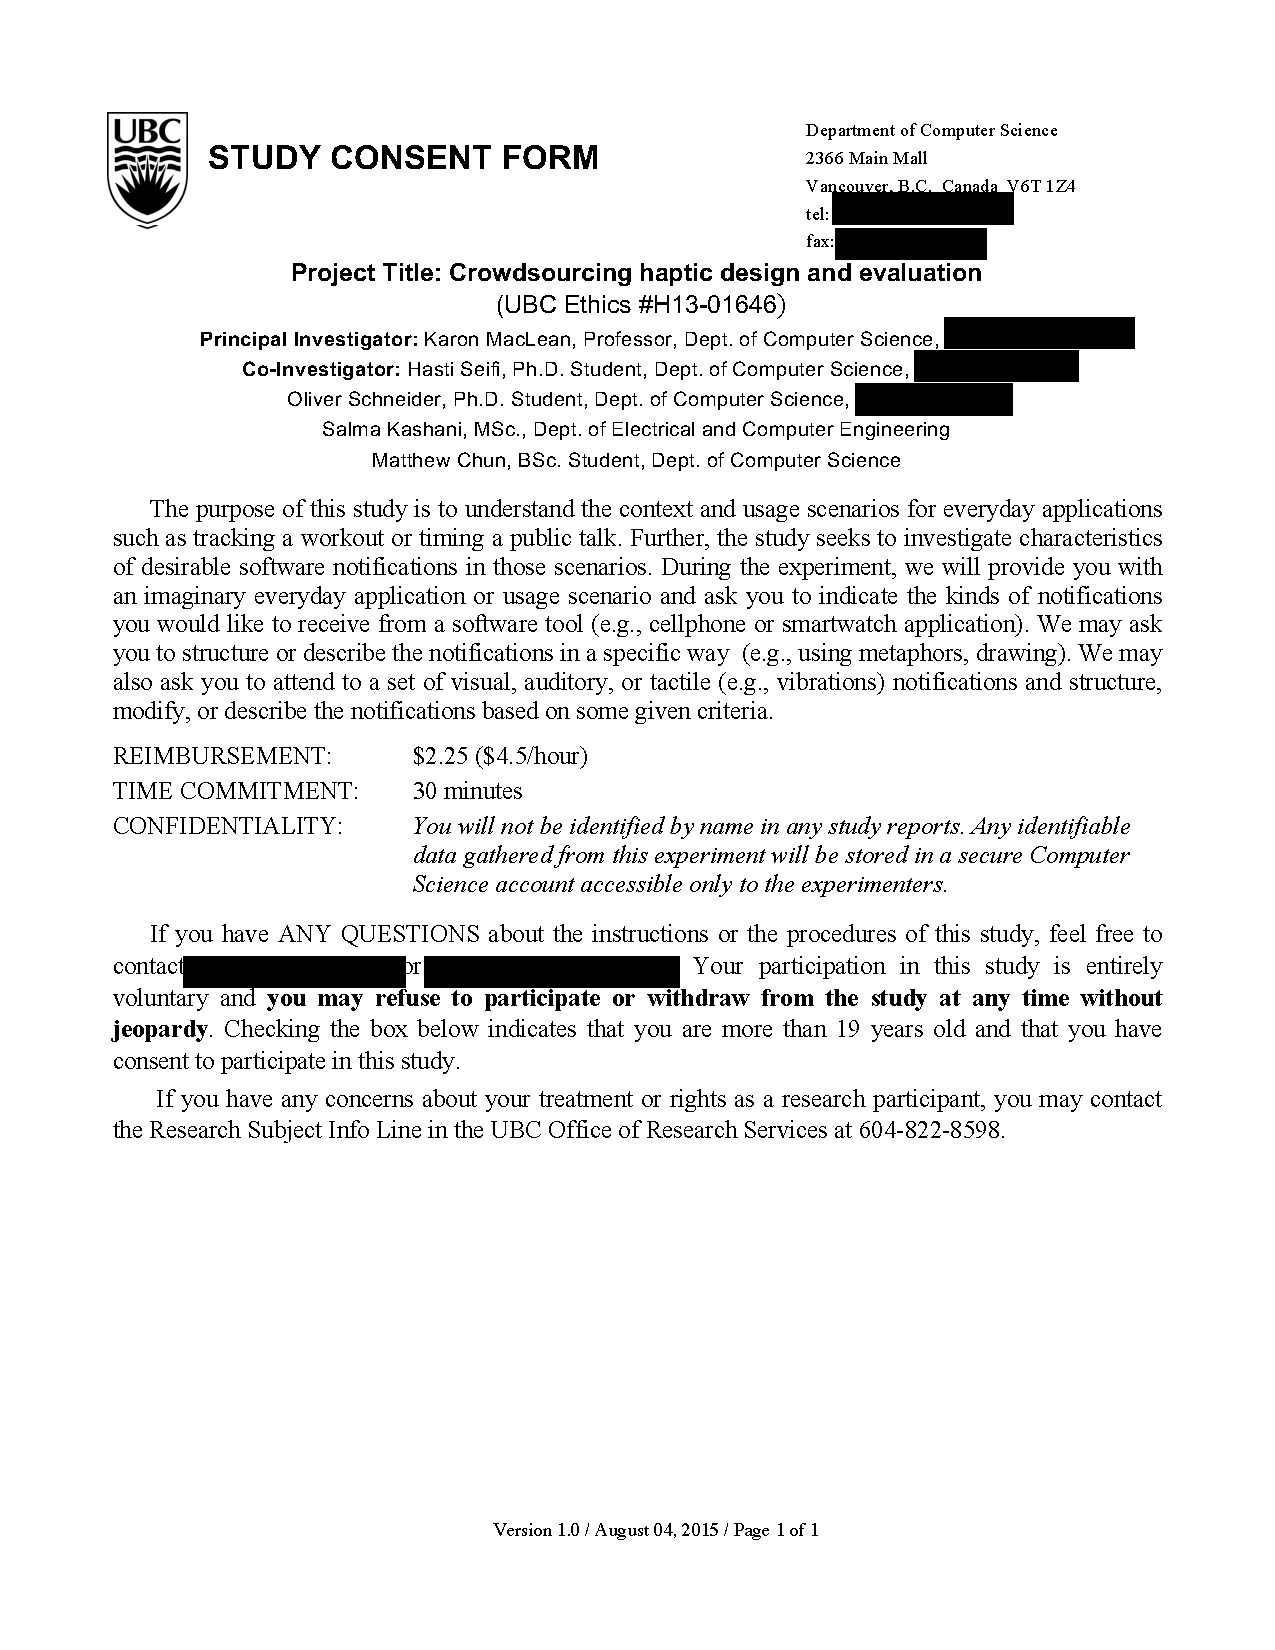
\includepdf[pages=-, pagecommand=\thispagestyle{plain}, width=1.25\textwidth]{Chapter99-SupportingMaterials/HSEthics/HapTurk-fromHS/HapTurk-Consent-v01-anon}
	

	%HandsOn interviews
	\subsection{HandsOn Forms}
	\label{ch:SupportingMaterials:ConsentForms:HandsOn}
	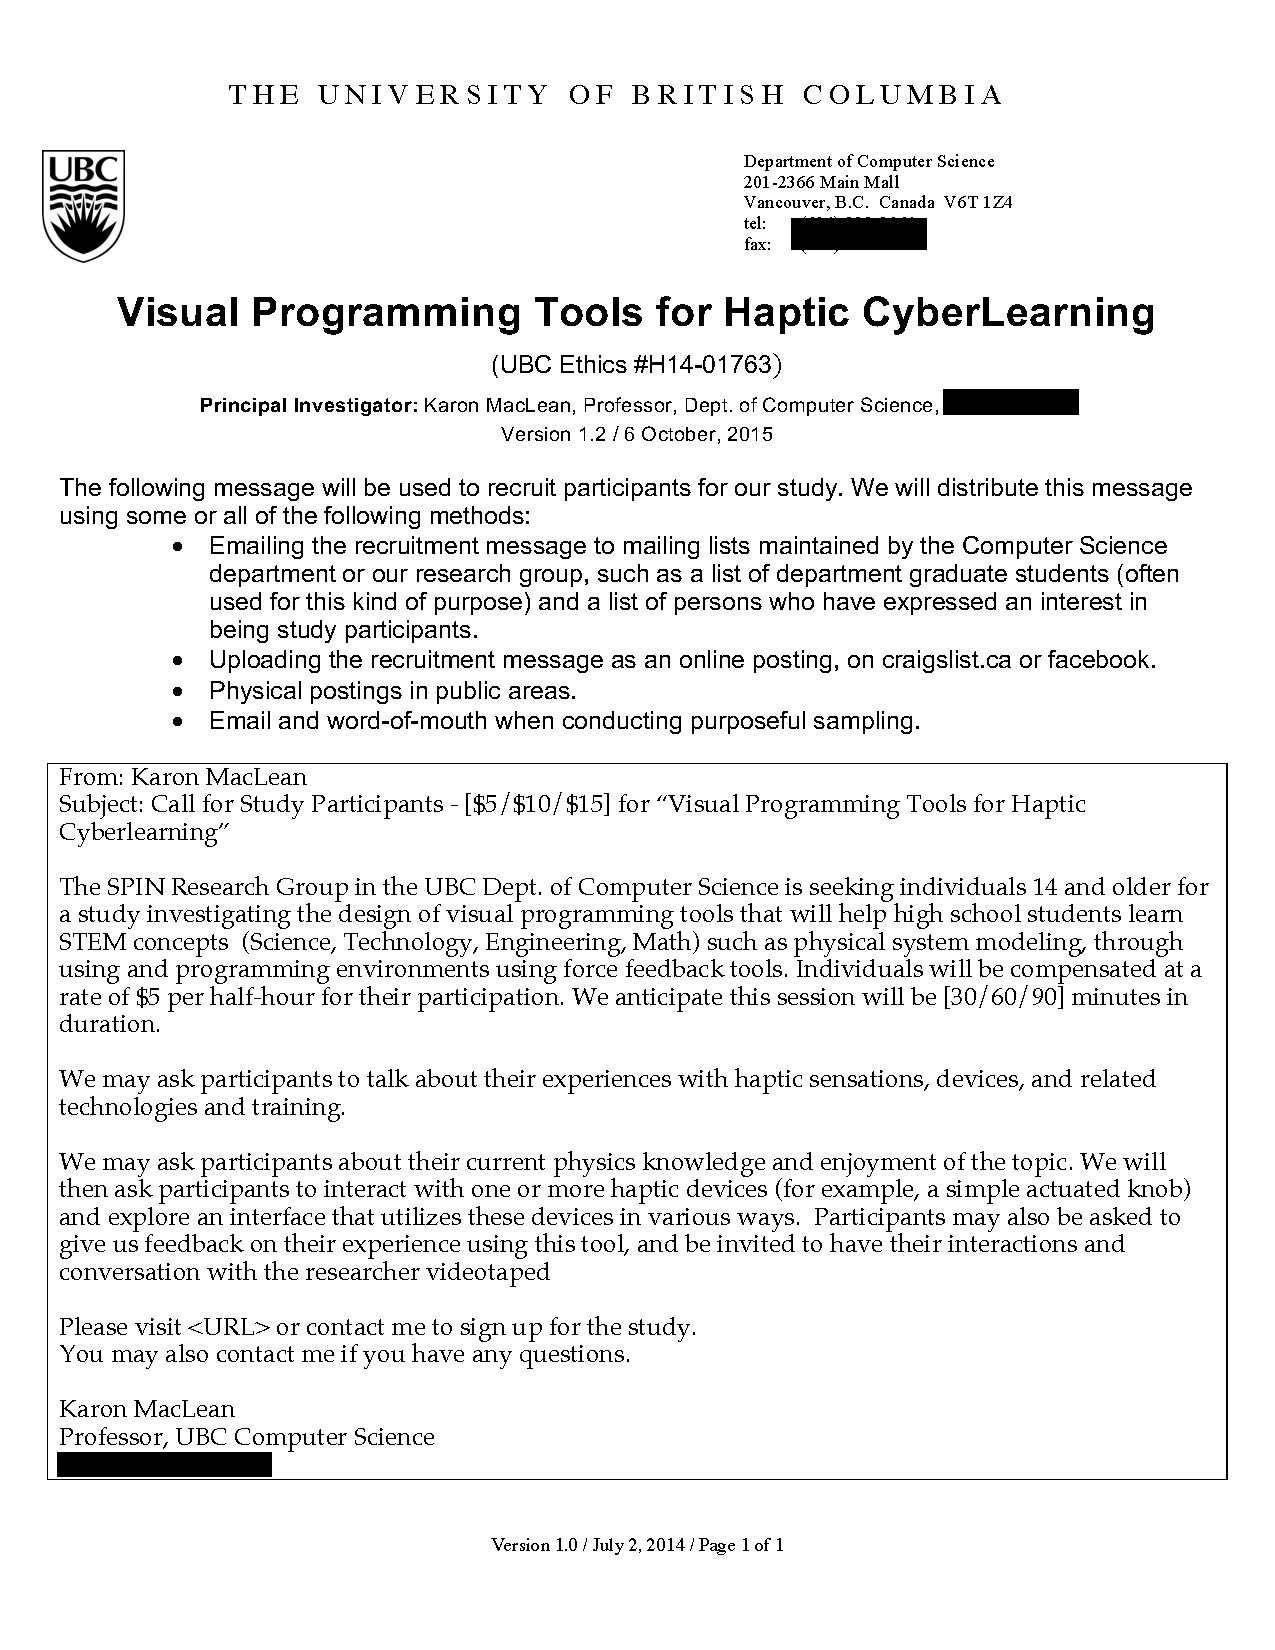
\includepdf[pages=-, pagecommand=\thispagestyle{plain}, width=1.25\textwidth]{Chapter99-SupportingMaterials/HandsOnEthics/CyberHapUsability-CallForParticipationEmail-v12-2015-10-06-onepage-anon}
	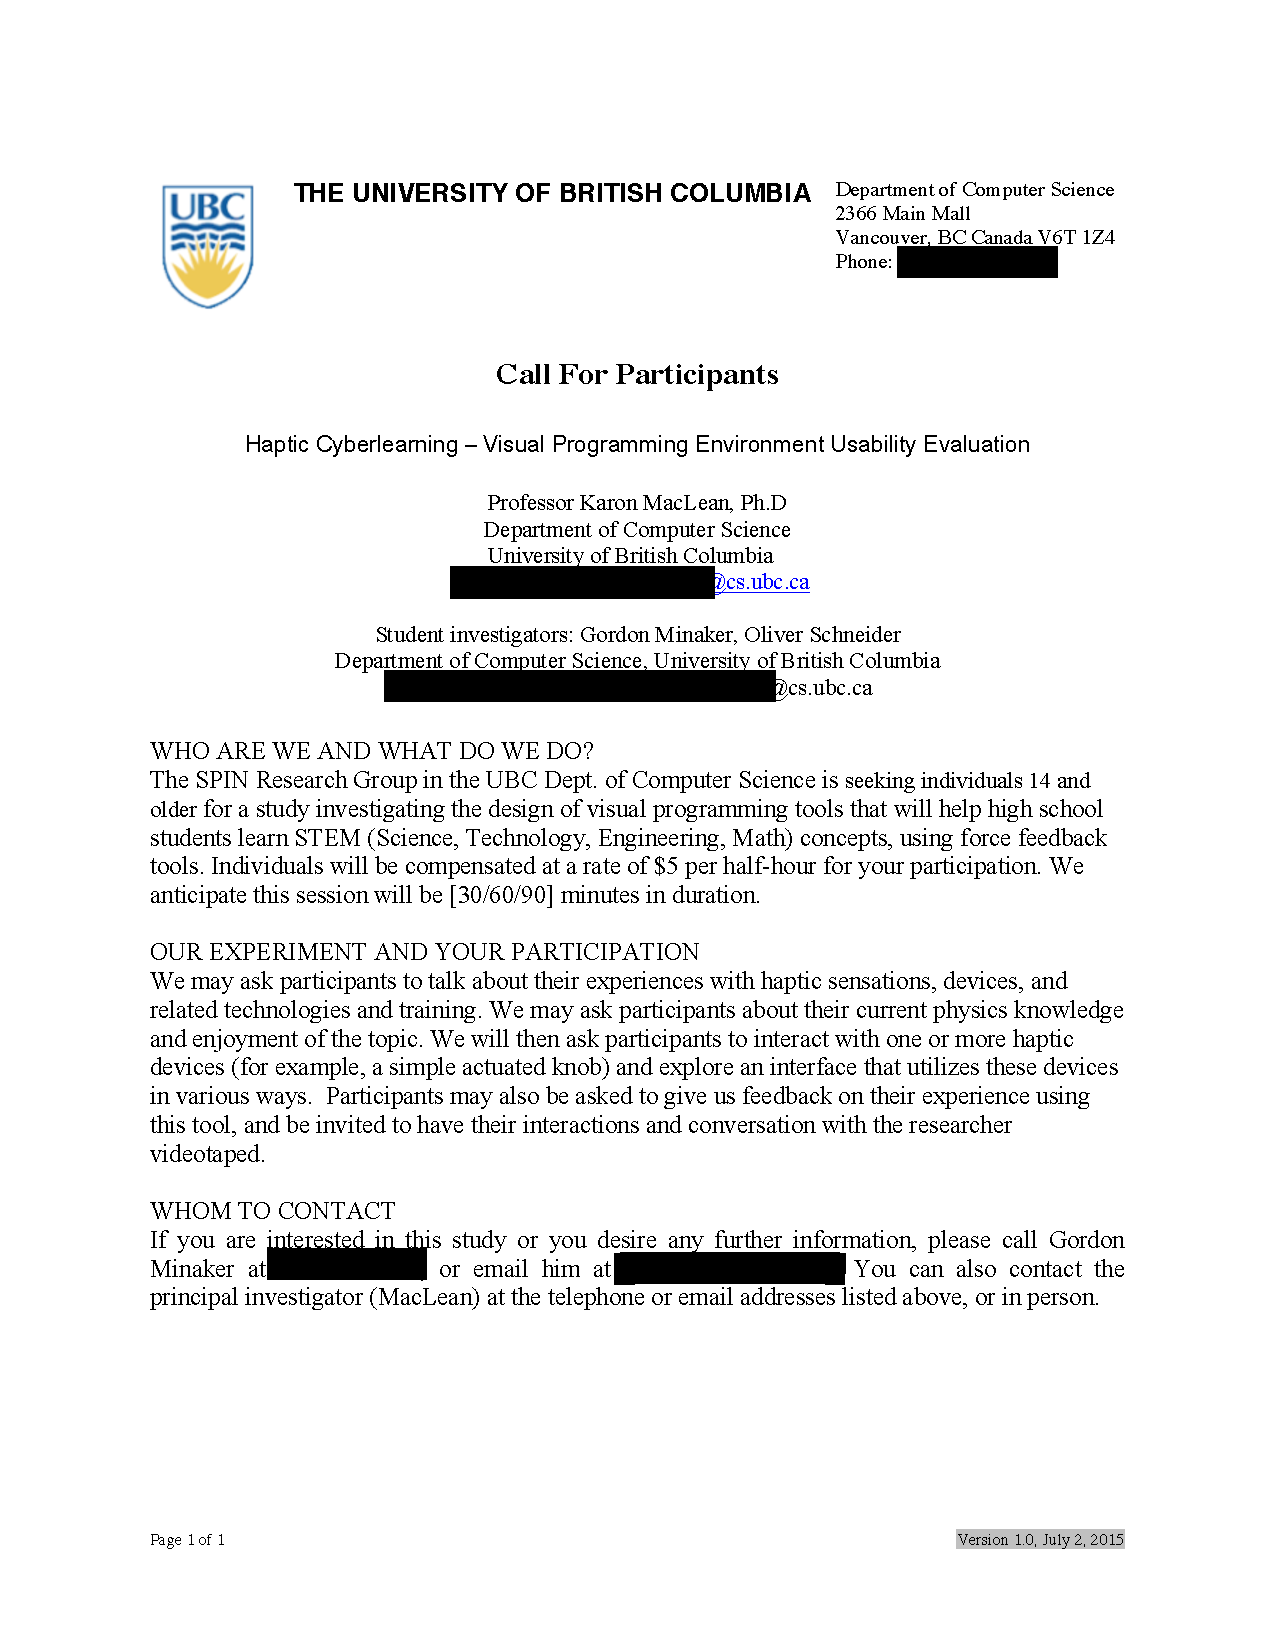
\includepdf[pages=-, pagecommand=\thispagestyle{plain}, width=1.25\textwidth]{Chapter99-SupportingMaterials/HandsOnEthics/CyberHapUsability-CallForParticipationPoster_v12_2015-10-06-anon}
	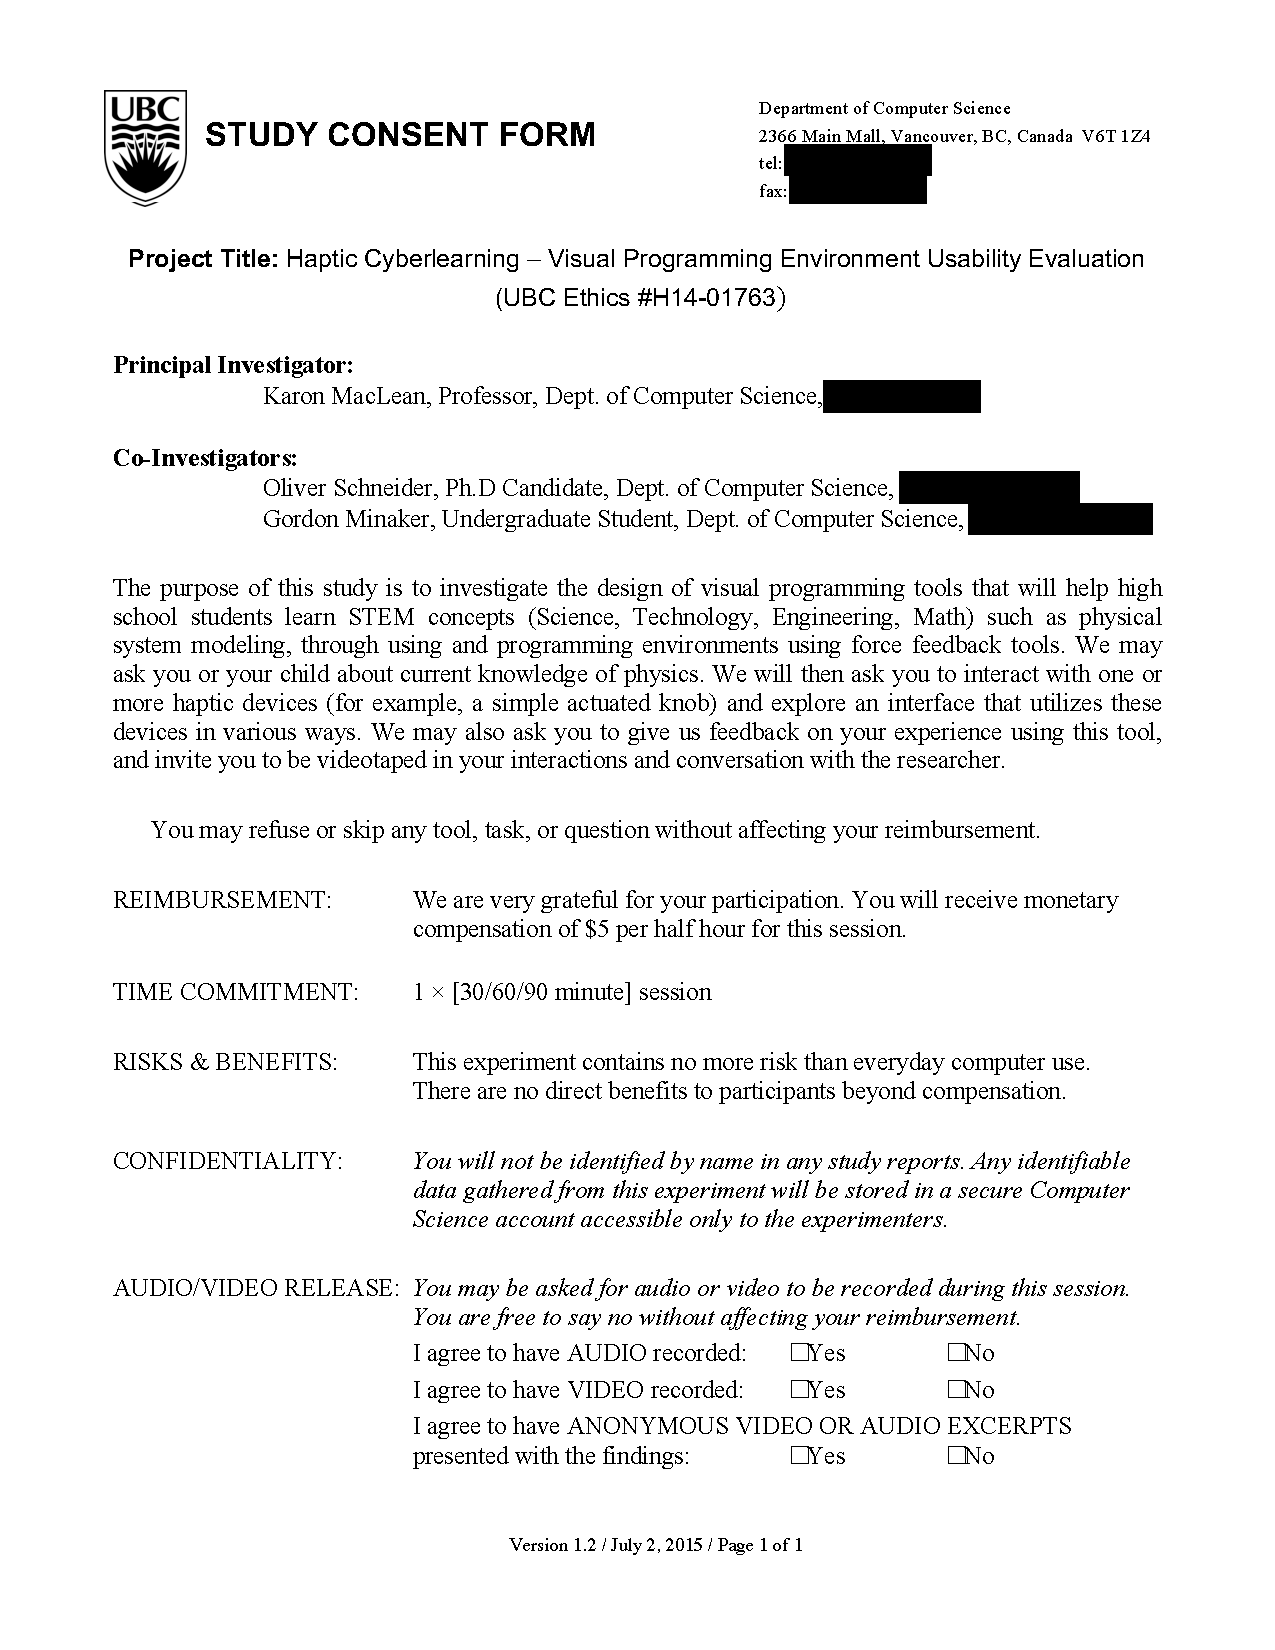
\includepdf[pages=-, pagecommand=\thispagestyle{plain}, width=1.25\textwidth]{Chapter99-SupportingMaterials/HandsOnEthics/CyberHapUsability-Consent-v13-2015-10-01-anon}
	
\includepdf[pages=-, pagecommand=\thispagestyle{plain}, width=1.25\textwidth]{Chapter99-SupportingMaterials/HandsOnEthics/CyberHapUsability-RequestForFollowup-v10-2014-07-02-anon}



	%haptician interviews
	\subsection{Haptician Interview Form}
	\label{ch:SupportingMaterials:ConsentForms:Haptician}
	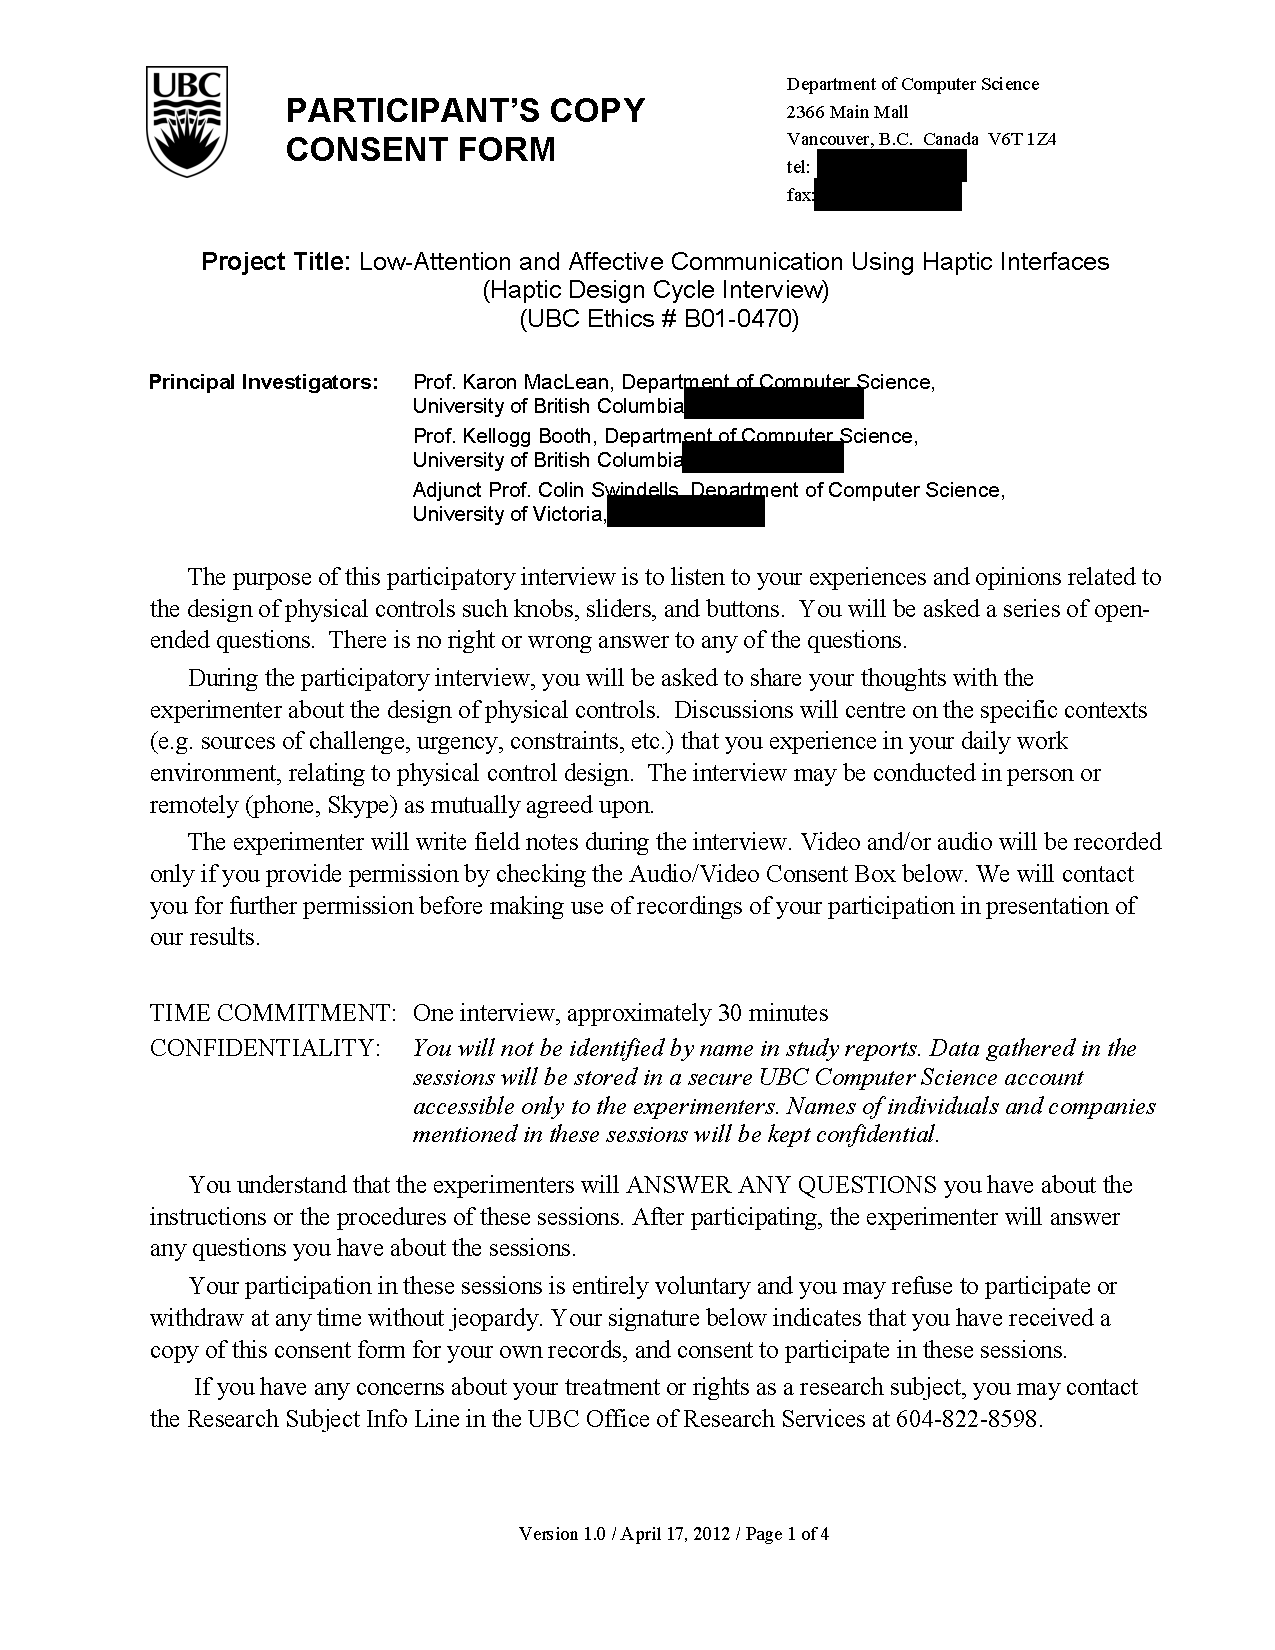
\includepdf[pages=-, pagecommand=\thispagestyle{plain}, width=1.25\textwidth]{Chapter99-SupportingMaterials/MainEthics/2012_04_17_DesignCycle-Consent_v10-anon}


\section{Examples of Qualitative Analysis Methods}
\label{ch:SupportingMaterials:MethodExamples}

	\begin{figure}[htbp] %  figure placement: here, top, bottom, or page
	   \centering
	   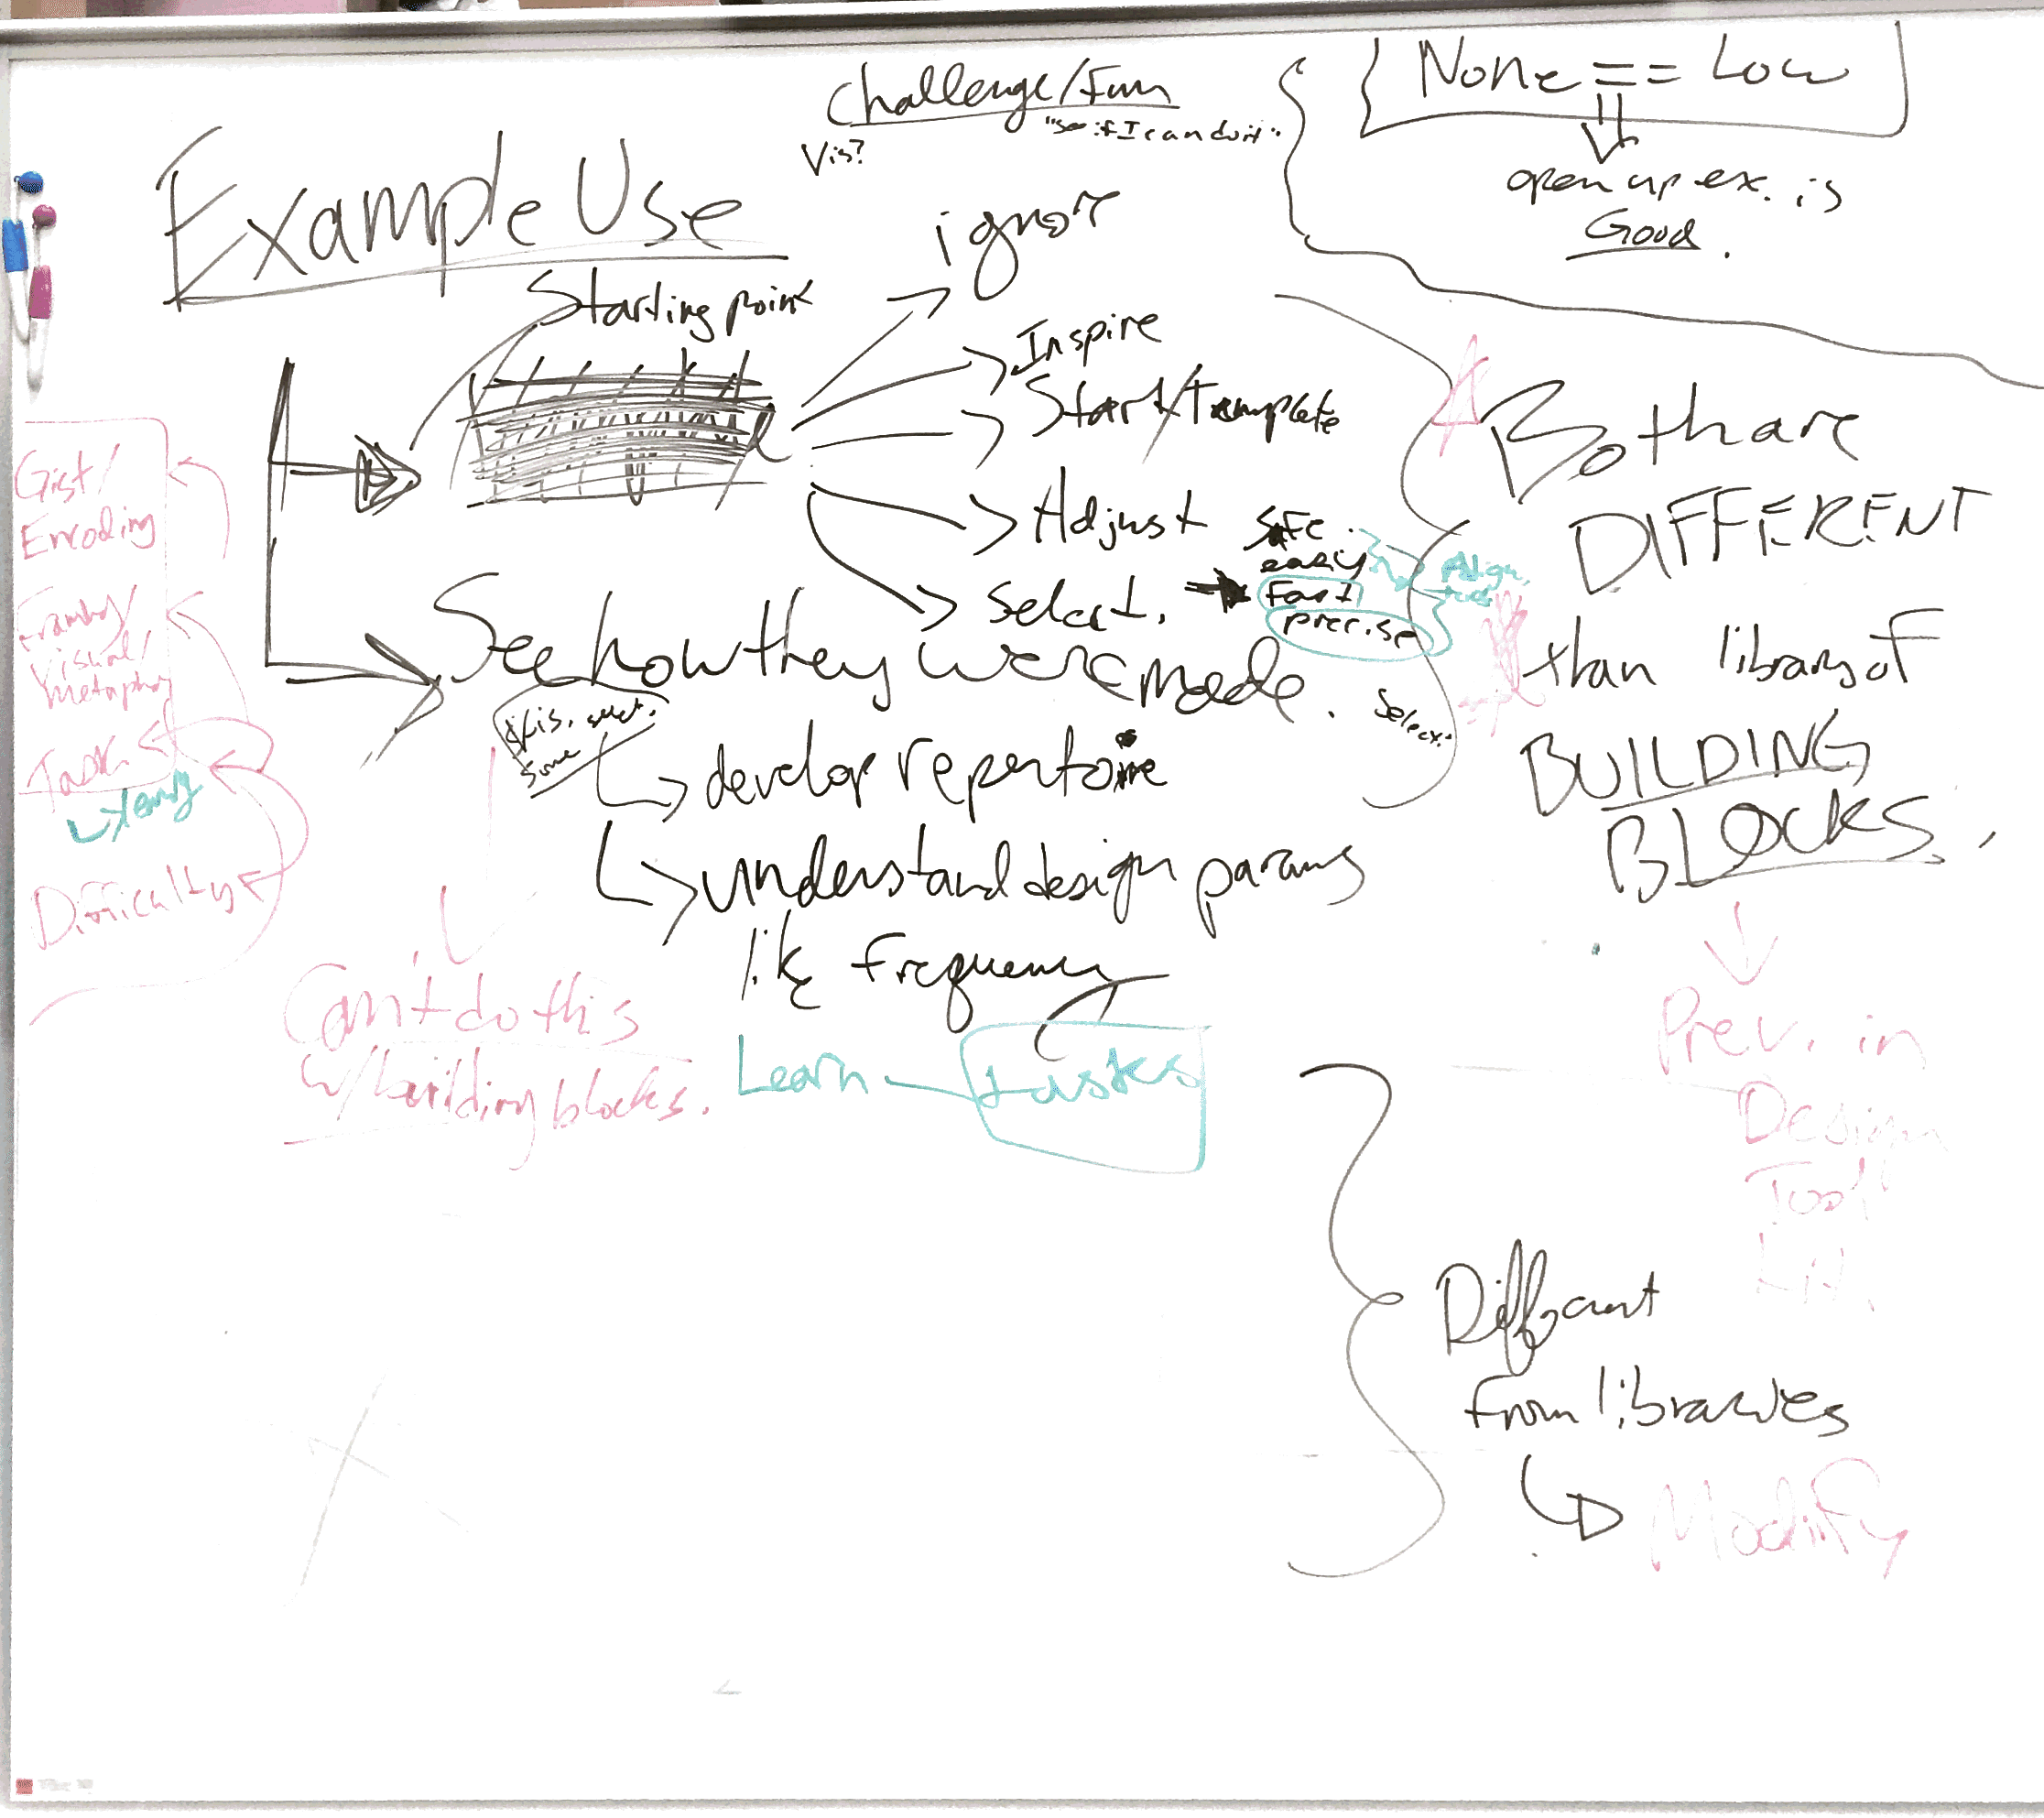
\includegraphics[height=\textwidth,angle=90]{Chapter99-SupportingMaterials/MethodExamples/MacaronAnalysisWhiteboard} 
	   \caption{Picture of whiteboard when developing themes during Macaron (\autoref{ch:macaron}) analysis.}
	   \label{fig:SupportingMaterials:MethodExamples:MacaronAnalysisWhiteboard}
	\end{figure}
	
	
	\begin{figure}[htbp] %  figure placement: here, top, bottom, or page
	   \centering
	   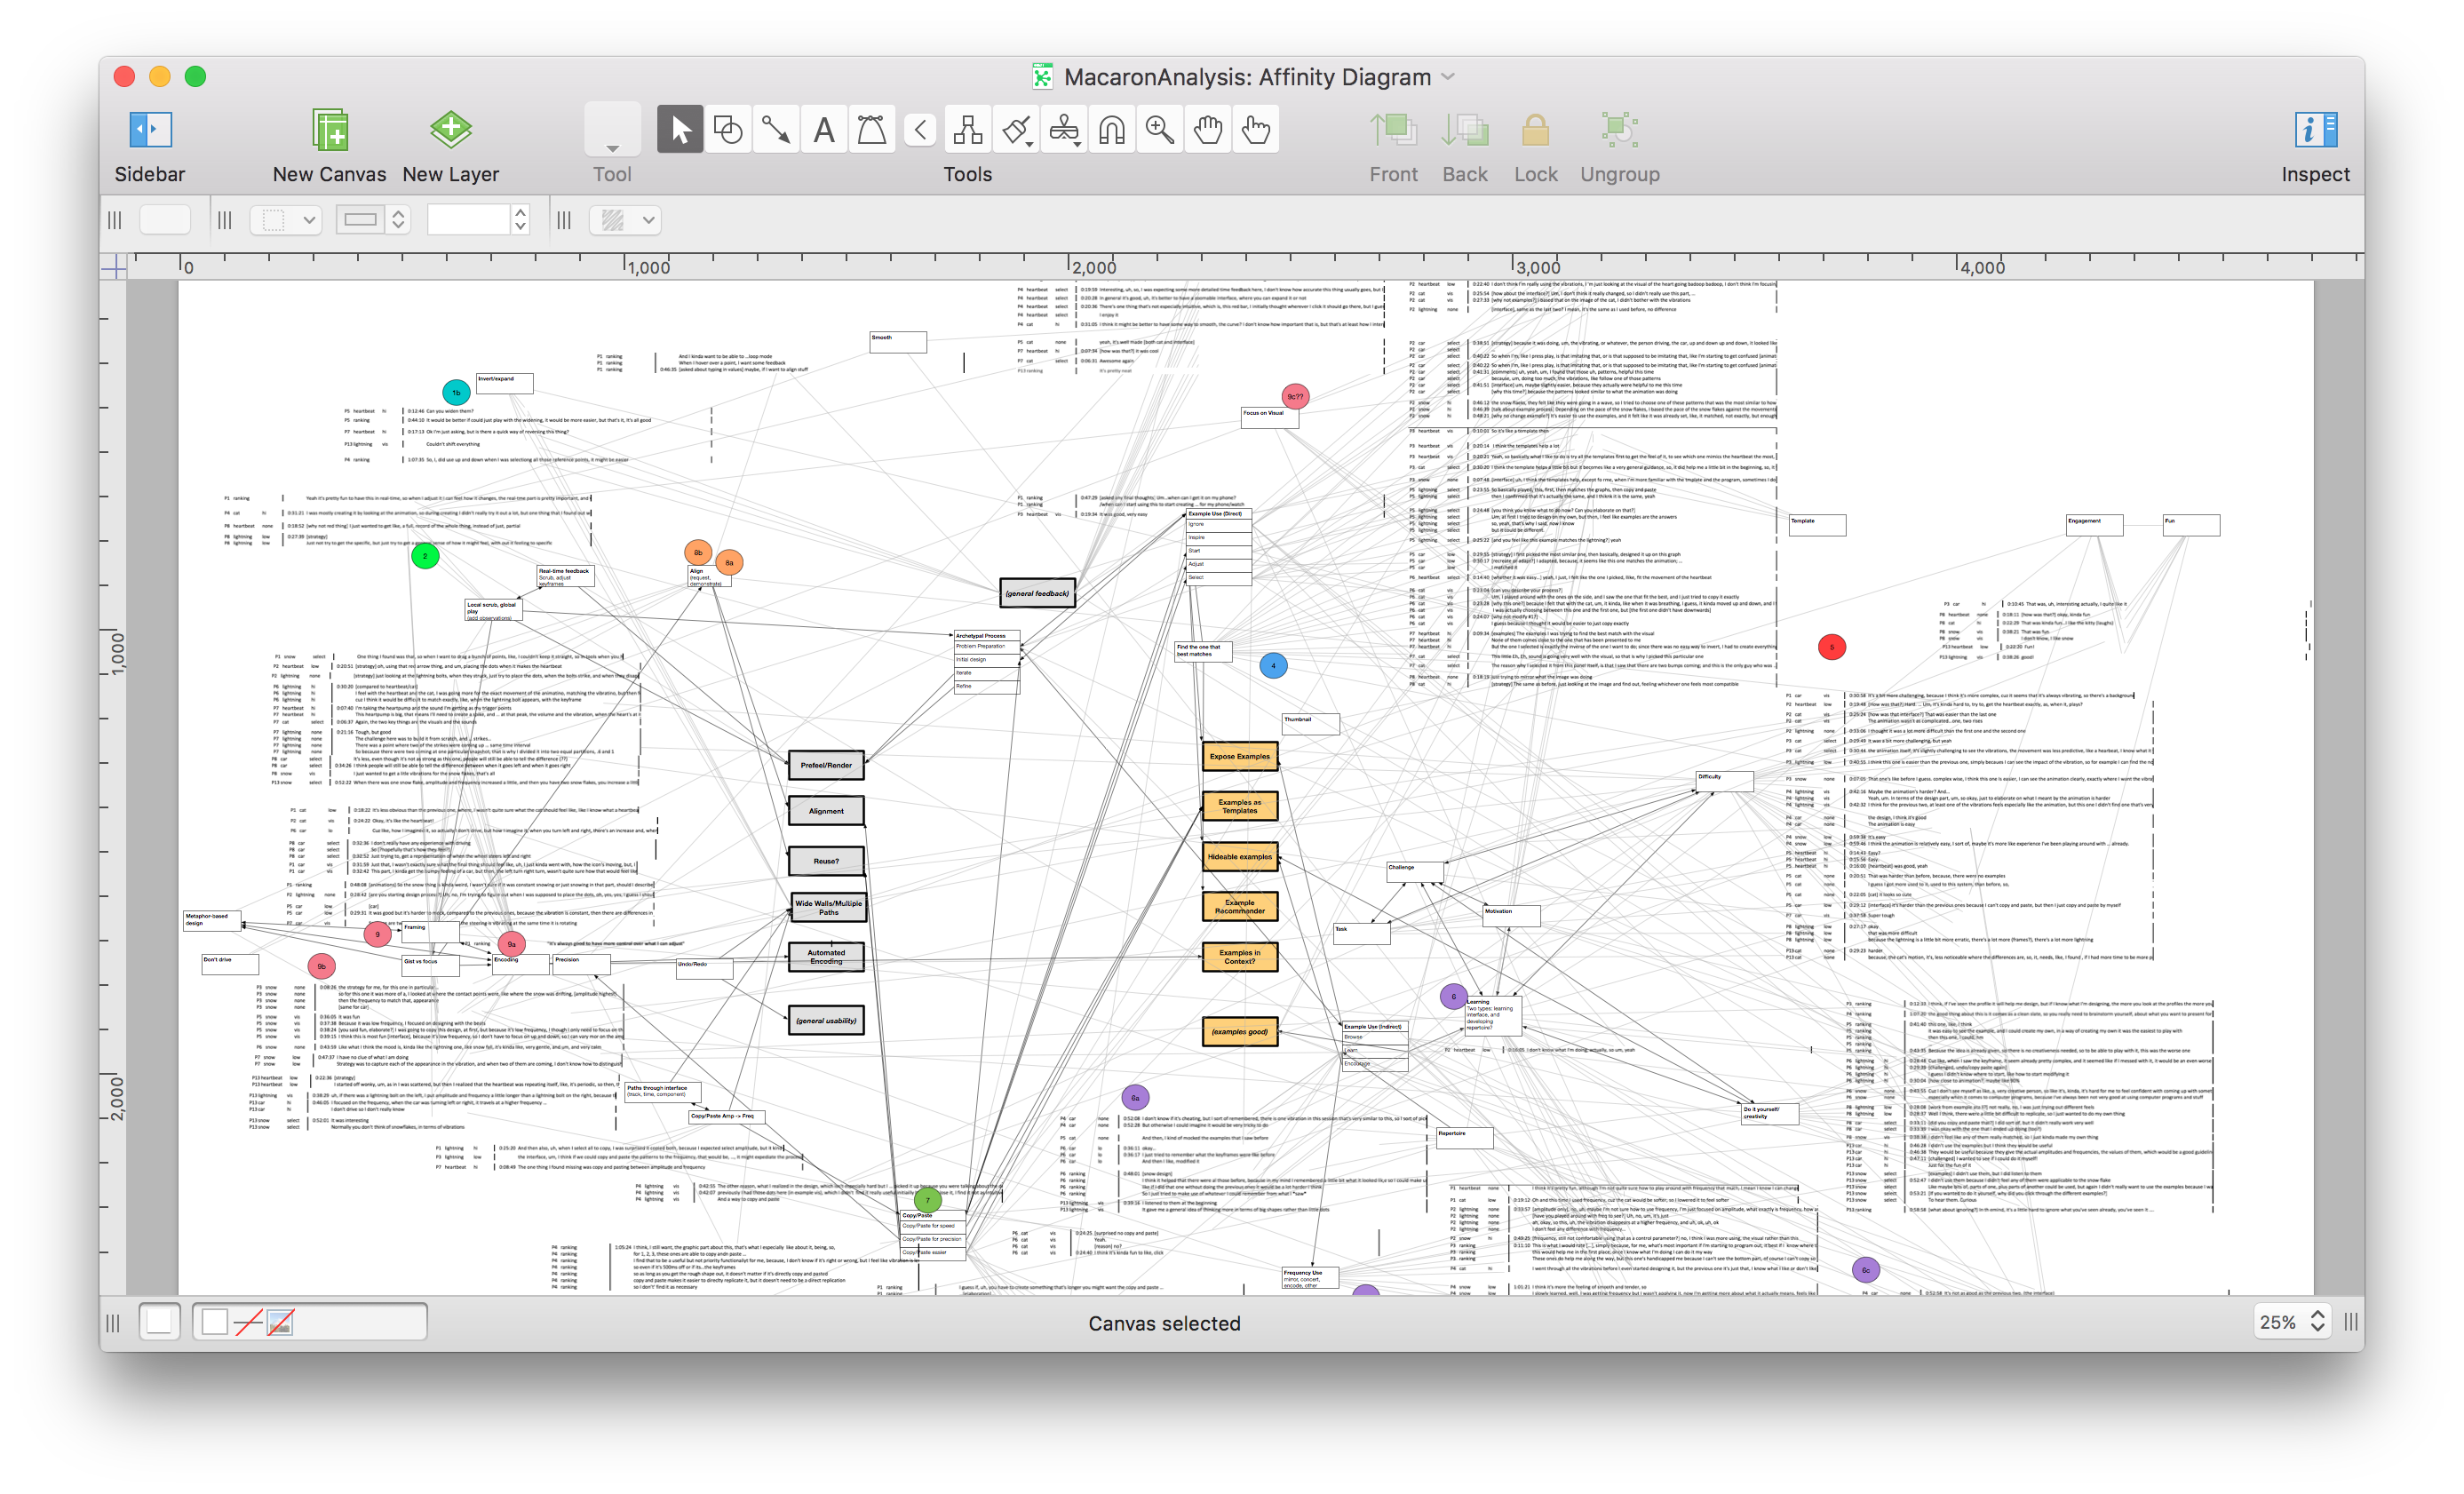
\includegraphics[width=0.9\textheight,angle=90]{Chapter99-SupportingMaterials/MethodExamples/MacaronClustering} 
	   \caption{Affinity diagram showing clustering of participant statements into themes during Macaron (\autoref{ch:macaron}) analysis.}
	   \label{fig:SupportingMaterials:MethodExamples:MacaronClustering}
	\end{figure}

	\begin{figure}[htbp] %  figure placement: here, top, bottom, or page
	   \centering
	   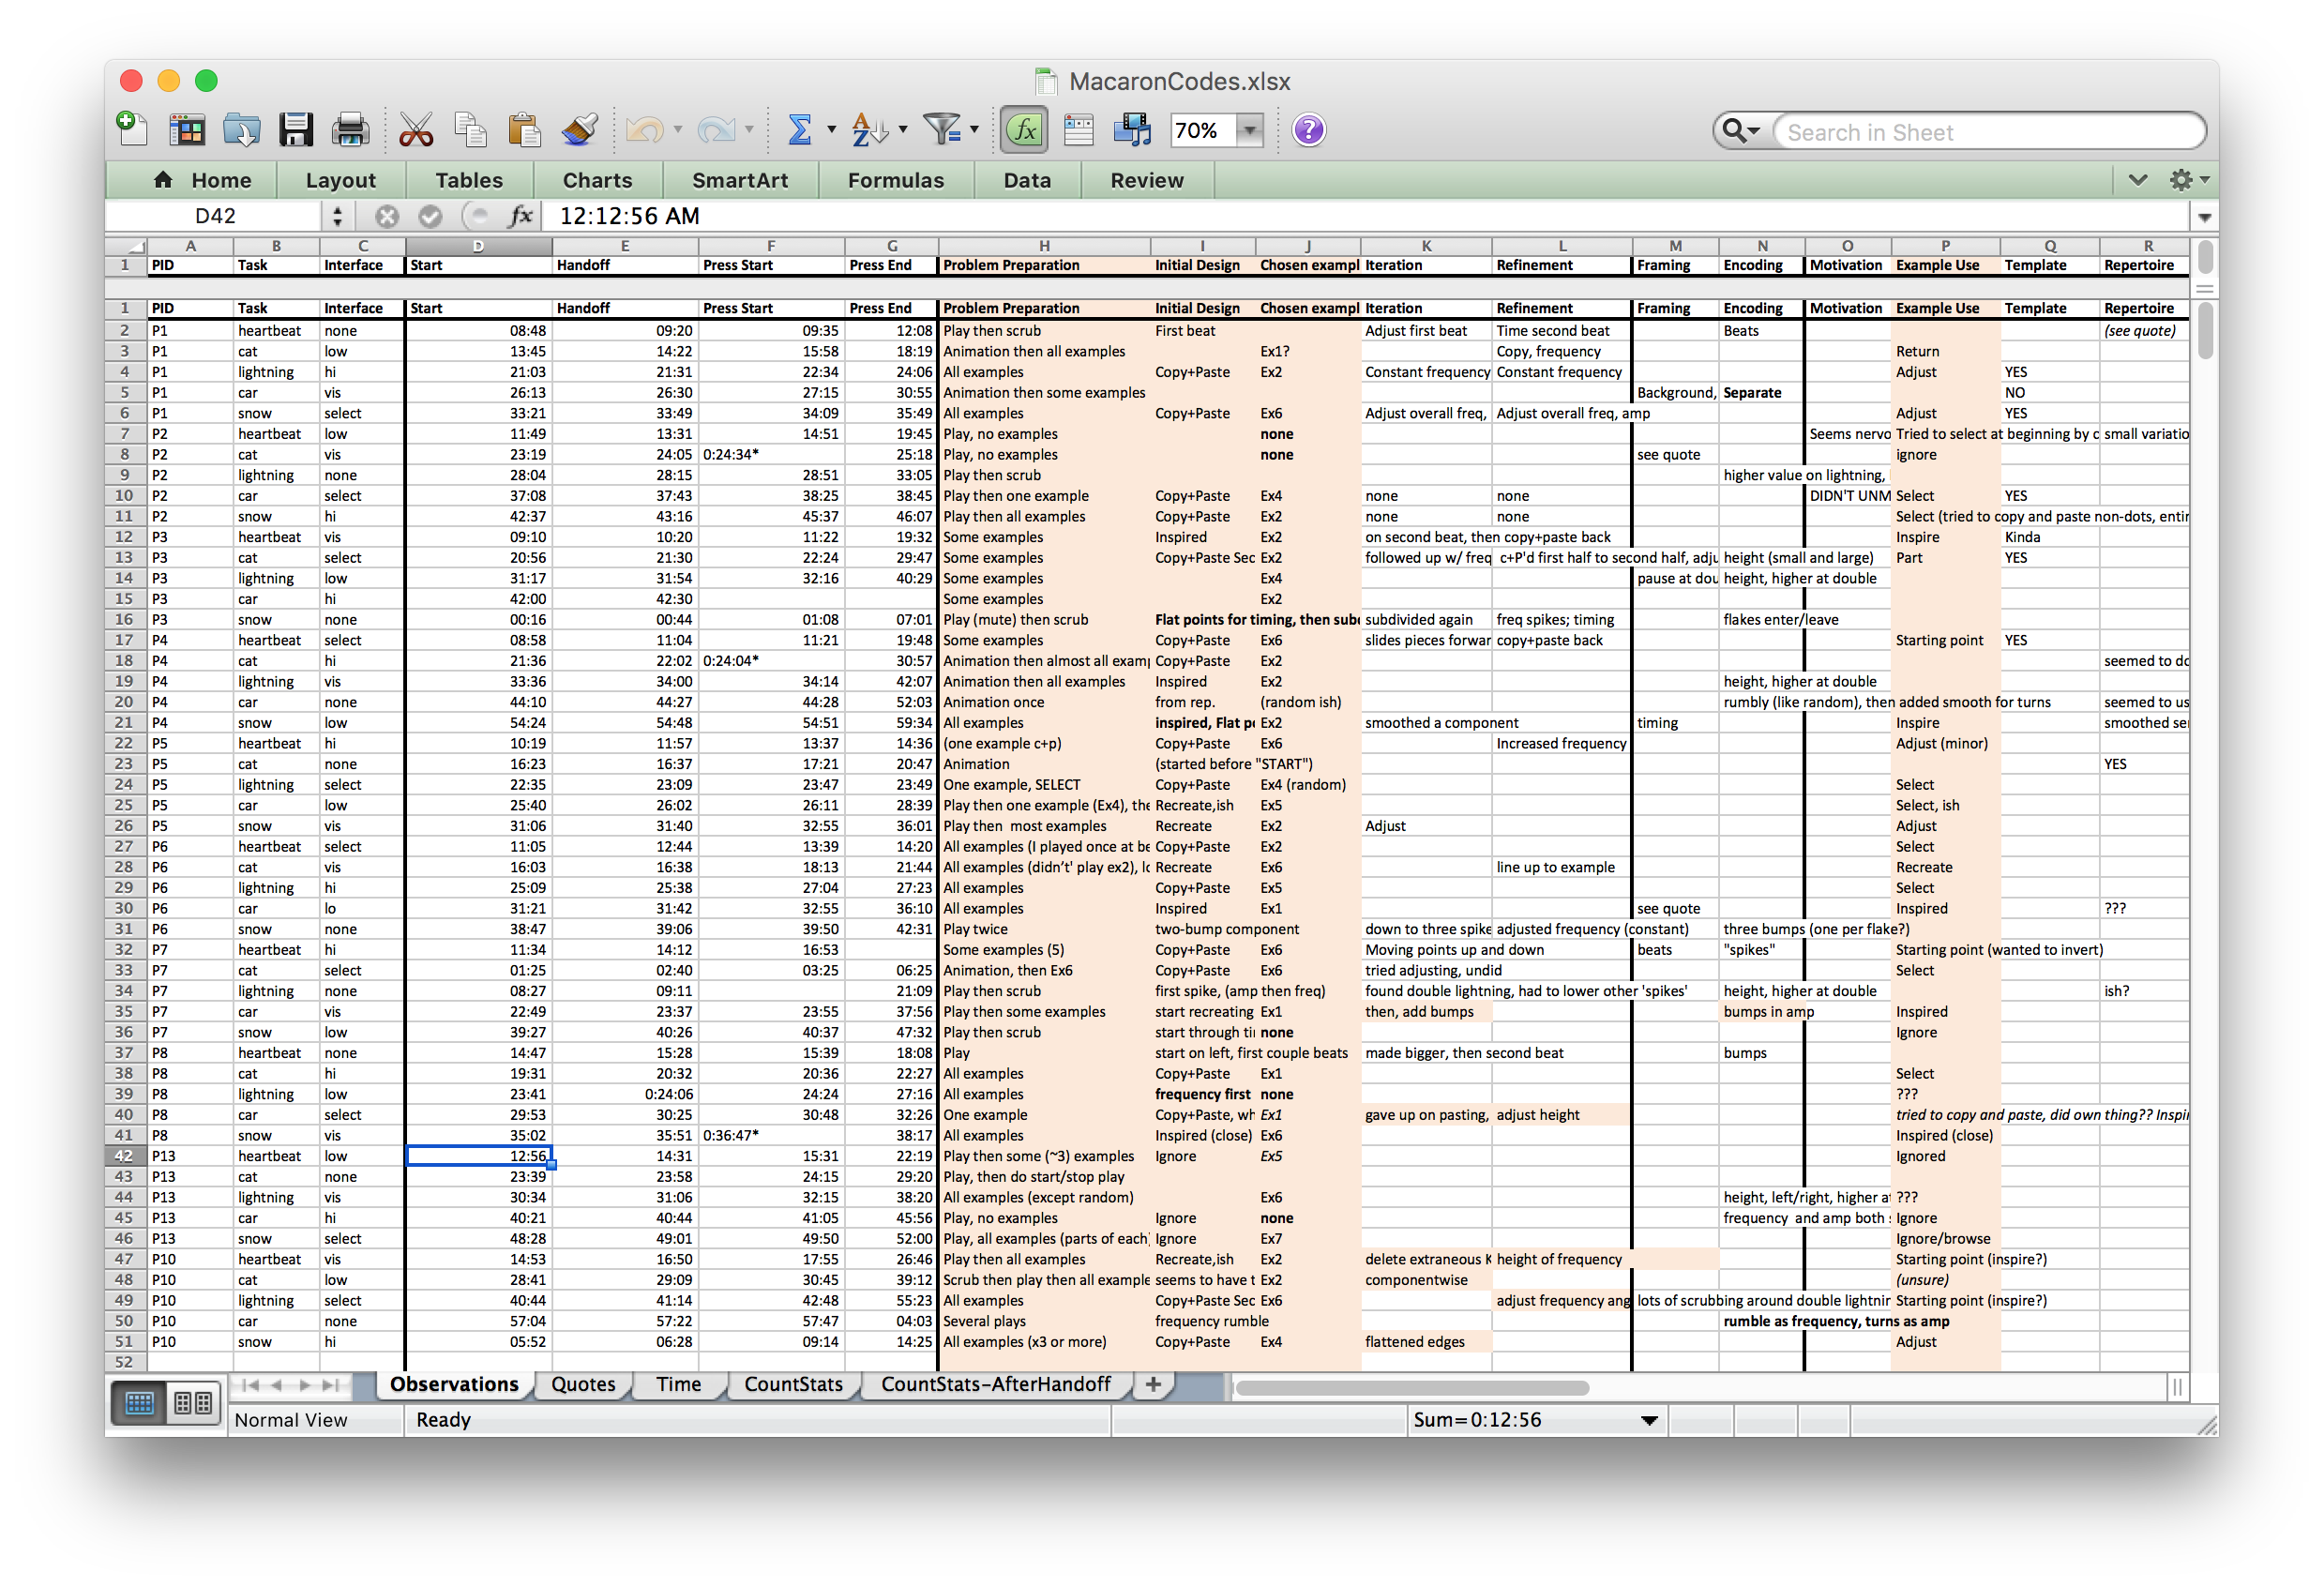
\includegraphics[width=0.9\textheight,angle=90]{Chapter99-SupportingMaterials/MethodExamples/MacaronCoding} 
	   \caption{Screenshot of video coding sheet used to develop and count codes and calculate task timing during Macaron (\autoref{ch:macaron}) analysis.}
	   \label{fig:SupportingMaterials:MethodExamples:MacaronCoding}
	\end{figure}


	\begin{figure}[htbp] %  figure placement: here, top, bottom, or page
	   \centering
	   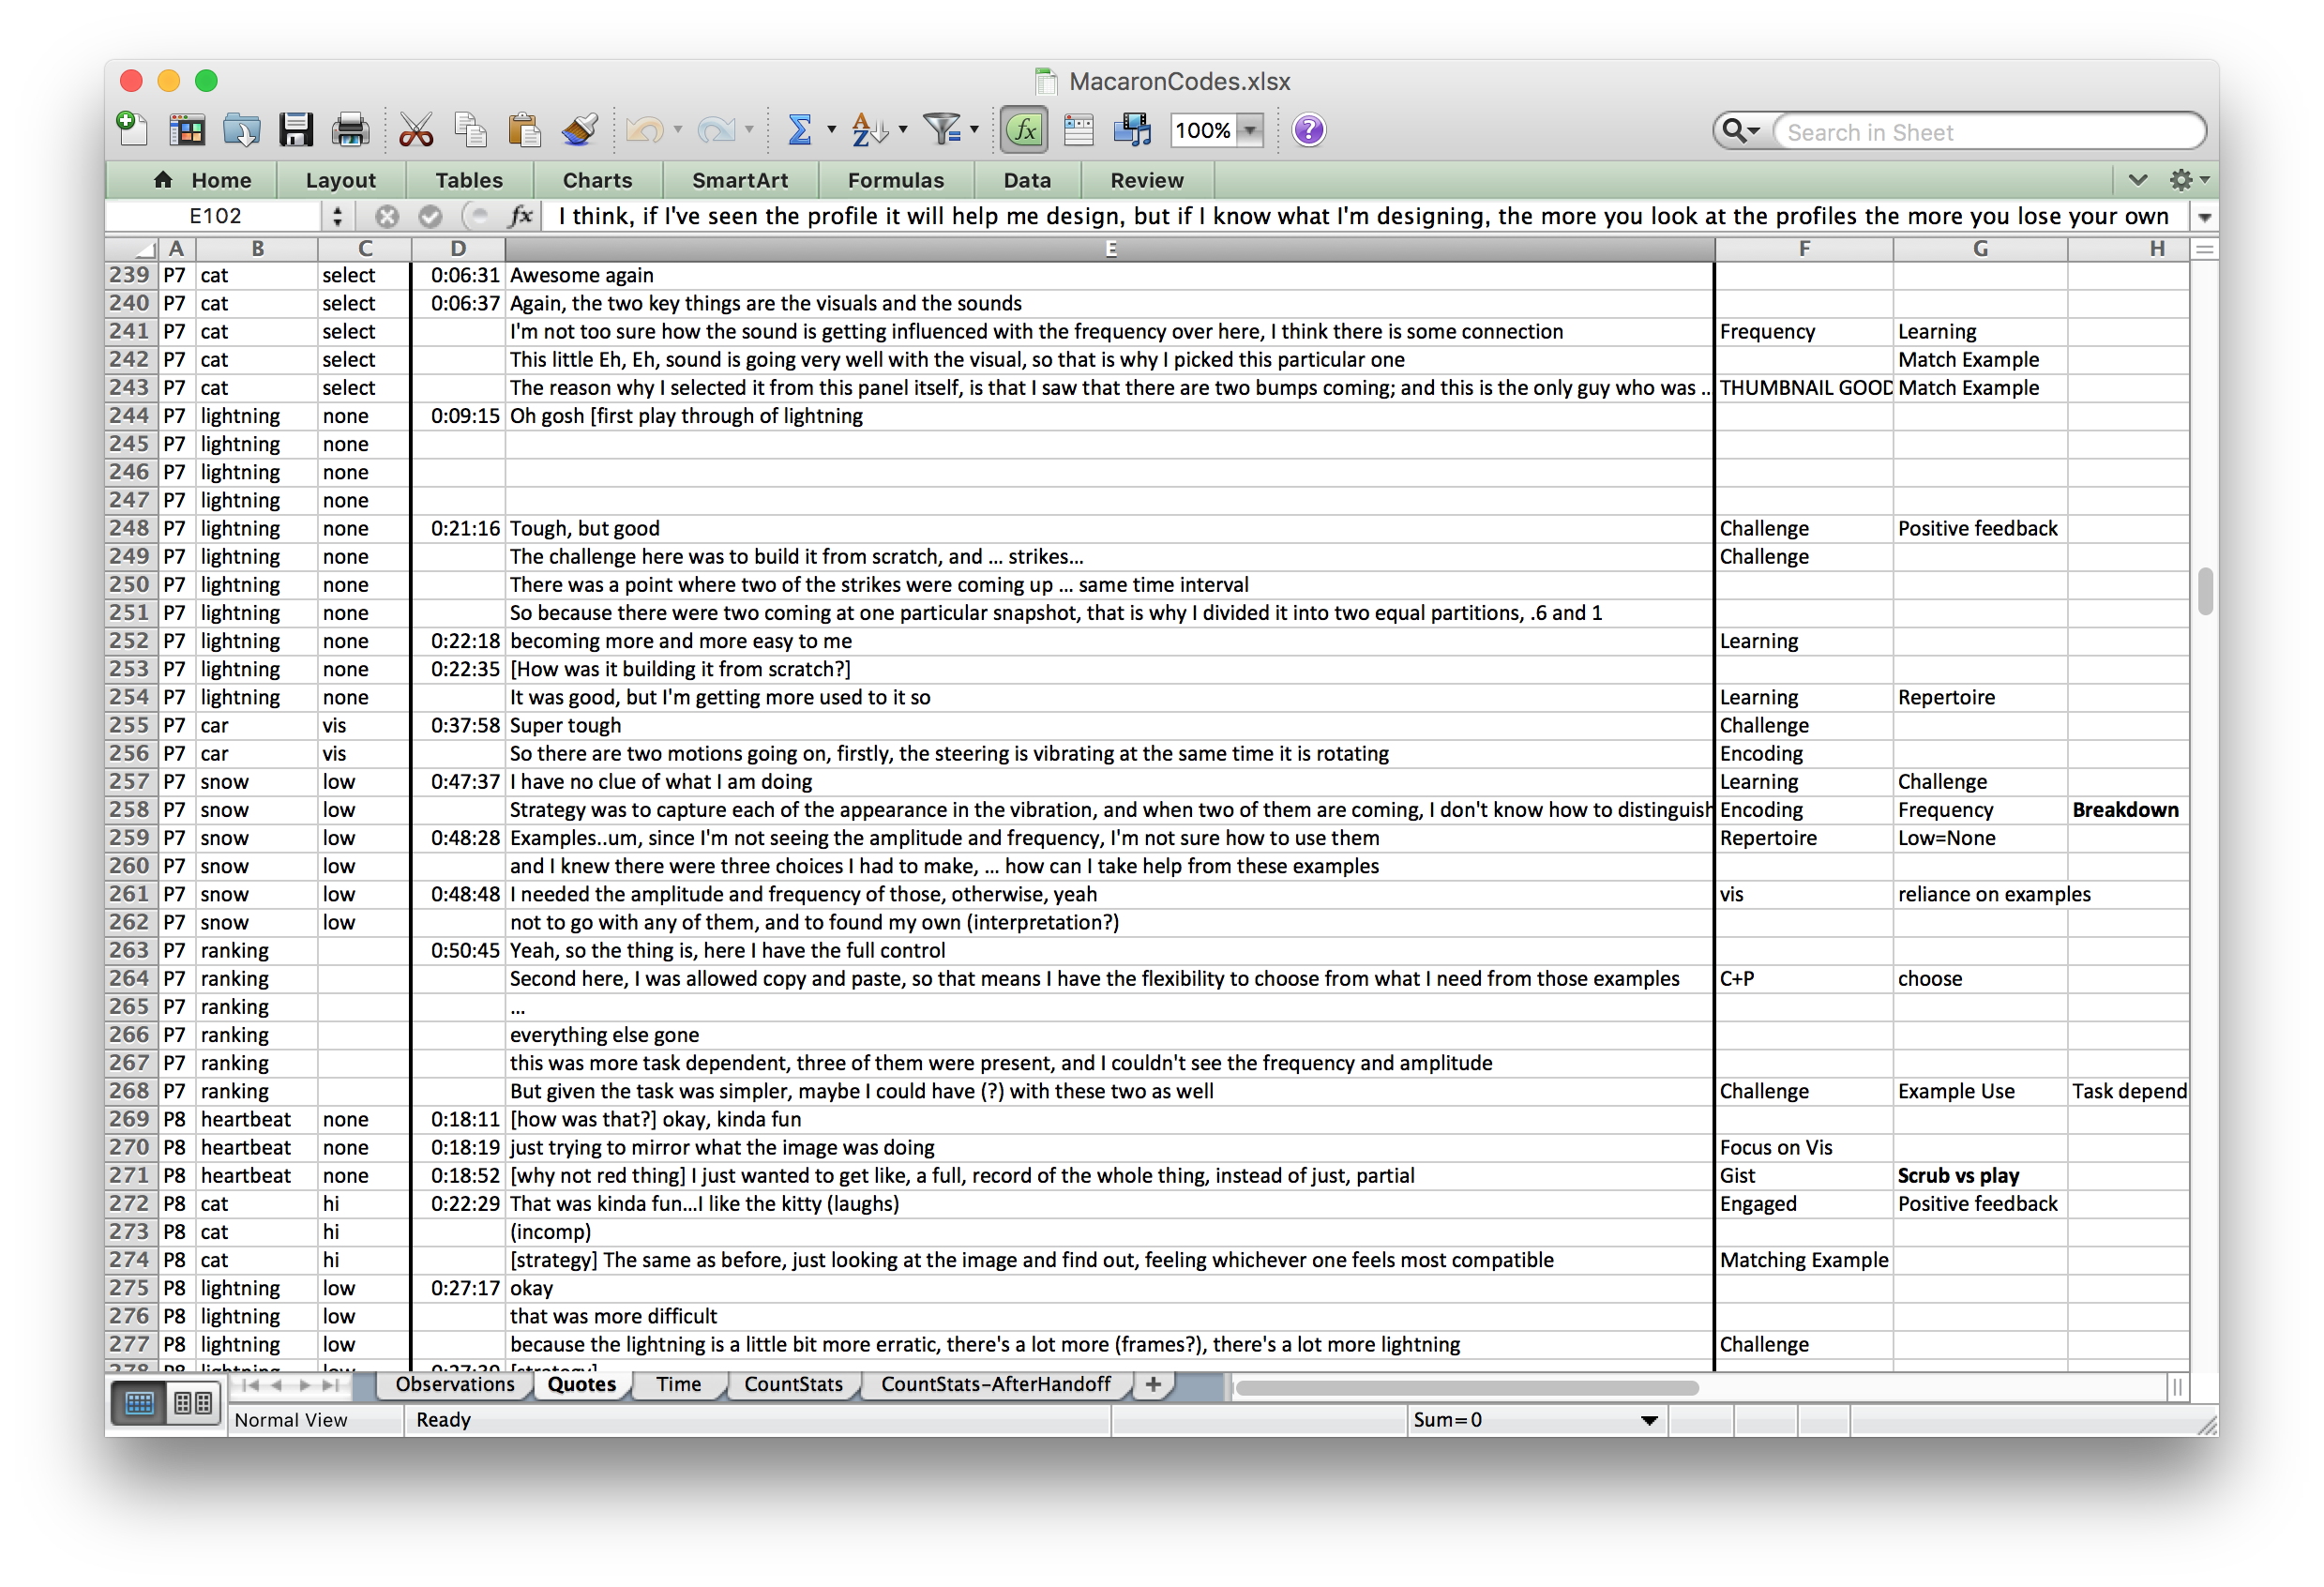
\includegraphics[width=0.9\textheight,angle=90]{Chapter99-SupportingMaterials/MethodExamples/MacaronQuotes} 
	   \caption{Screenshot of transcribed participant comments with code tags from Macaron (\autoref{ch:macaron}) analysis.}
	   \label{fig:SupportingMaterials:MethodExamples:MacaronQuotes}
	\end{figure}





\endinput